\documentclass[
	pdftex,
	a4paper, 
	oneside,
	parskip=half,
	headsepline,
	12pt
]{article}

\usepackage {a4wide}
\usepackage [utf8]{inputenc} % Zeichensatz, ermglicht die direkte Eingabe von Umlauten im Editor
\usepackage {fixltx2e} %korrigiert Fehler in LaTeX
\usepackage {fix-cm} %korrigiert Fehler in Standard-Schriften
\usepackage [T1] {fontenc} %Ausgabecodierung
\usepackage {textcomp} %Sonderzeichen
%\usepackage [ngerman] {babel} %Sprachunterstützung
\usepackage [english] {babel} %Sprachunterstützung
\usepackage [automark, autooneside, headsepline]{scrpage2}
\usepackage [pdftex]{graphicx} % Einbindung von Grafiken (pdf, png, jpg)
\usepackage {fixmath}
\usepackage {subfigure}
\usepackage {amsmath}
\usepackage {amssymb}
\usepackage {listings}
\lstdefinelanguage{tcl}{
moredelim=**[is][\itshape]{<kursiv>}{</kursiv>}
}
\lstset{language=tcl, basicstyle=\footnotesize\ttfamily}
\usepackage {chngcntr}
\usepackage{pdfpages}
\usepackage{hyperref}

\renewcommand {\thefigure} {\thesection.\arabic{figure}} %Sektionsnummer mit in Abbildungsnummer
\numberwithin {figure} {section} %Abbildungsnummer mit jeder Sektion zurücksetzen
\renewcommand {\thetable} {\thesection.\arabic{table}} %Sektionsnummer mit in Tabellennummer
\renewcommand {\theequation} {\thesection.\arabic{equation}} %Sektionsnummer mit in Formelnummer
\numberwithin {equation} {section} %Formelnummer mit jeder Sektion zurücksetzen
\counterwithout{table}{section}

\begin {document}
\pagestyle{empty}
\begin{titlepage}
\begin{figure}
  \begin{center}
    \hbox to \hsize{%
      \begin{tabular}[m]{c}
        Hochschule Ostfalia\\
        Fakultät Elektrotechnik \\
        Labor für Kommunikationssysteme \\
      \end{tabular}%
      \hfill%
\begin{tabular}[m]{c}
        
\includegraphics[width=7cm]{logo.jpg}
      \end{tabular}
    }
  \end{center}
\end{figure}

\begin{center}
\rule{0pt}{0pt}
\vfill
\vfill

\begin{huge}
%Studienarbeit\\[0.9ex]
AskoziaPBX-\\[0.75ex]
Performancetests\\[0.75ex]
%basierten Prozessorsystem\\[0.75ex]
\end{huge}

\vfill
\vfill
\vfill
\vfill
Written by\\
\vspace*{.5cm}
Mark Stephan\\
\vspace{.5cm}
%xx. Monat 20xx -- xx. Monat 20xx \\

\vfill
\vfill
\vfill
\vfill
\vfill
\vfill
\vfill

\begin{tabular}{rl}
Head:    & Prof. Dr.-Ing. D. Wermser\\
Supervisor:   & M. Iedema, B.Sc.\\
\end{tabular}
\end{center}
23.07.2010
\end{titlepage}

\cleardoublepage
\pagestyle{empty}
\tableofcontents
\pagestyle{empty} 
%\listoffigures
\newpage
%\pagestyle{empty}
%\listoftables
%\pagestyle{empty}
\lstlistoflistings
\pagestyle{plain}
\setcounter{page}{1}
\pagenumbering{arabic}

\section{Introduction}
\label{sec:introduction}

This subproject of AskoziaPBX was developed for executing performance- and stress-tests to different Askozia-boxes.
It was written by Mark Stephan \newline (mark.stephan@askozia.com) during a job as a student
assistant for the Askozia-founder Michael Iedema (michael@askozia.com) in Spring/Summer 2010. 

It is very important to understand the differences between the three test-types (two-way-calls, conference calls with fixed number of
calls and conference calls with fixed number of rooms). It is explained detailed in the first paragraphs of chapters
\ref{sec:two-way}, \ref{sec:conf-call} and \ref{sec:conf-room}.

%%%%%%%%%%%%%%%%%%%%%%
\subsection{Problem}%%
%%%%%%%%%%%%%%%%%%%%%%
The AskoziaPBX software can be downloaded as firmware image for embedded systems and as live cd. The live cd can be run on every normal computer, so the underlying hardware may have very different performance. E.g., the same software can handle three, 30 or 300 parallel two-way-calls, depending on the computer performance. So we had to develop an algorithm to find out how tough the current Askozia box is.
 
%%%%%%%%%%%%%%%%%%%%%%%
\subsection{Features}%%
%%%%%%%%%%%%%%%%%%%%%%%
The current testsuite supports the following features:

\begin{itemize}
\item completely automatic testing of one AskoziaPBX
\item automatic configuration of the AskoziaPBX with the needed settings
\item three different types of test:
	\begin{description}
	\item [two-way-calls] The testsuite establishes a variable number of A-to-B (or end-to-end) calls between the AskoziaPBX and the testsystem. This test simulates normal telephone calls between two persons.
	
	\item [conference-tests with fixed number of calls] The testsuite calls a variable number of different conference rooms with a fixed number of users in each room.

	\item [conference-tests with fixed number of rooms] The testsuite calls a fix number of conference rooms with a variable number of users in each rooms.
	\end{description}
	
\item monitoring of the CPU-load of the AskoziaPBX caused by the testcalls
\item download of the recorded CPU-load data
\item interpretation and creation of graphs of the testresults 
\end{itemize}

%%%%%%%%%%%%%%%%%%%%
\subsection{Usage}%%
%%%%%%%%%%%%%%%%%%%%
The script can be called in the command line, e.g.: 

\begin{lstlisting}[breaklines=true,label=code:script-call,caption={Aufruf des Scripts} ]
./PERF_TEST <options>
perl PERF_TEST <options>
\end{lstlisting}

\begin{description}
\item {\texttt{-{}-local-ip=<IP>}} \newline
The IP-adress of the testcomputer that executes the testscript.
<IP> stands for the address of the device connected to the AskoziaPBX.
\newline Standard: undefined (\textbf{must} be defined)
\newline Example: \texttt{-{}-local-ip=192.168.0.2}

\item {\texttt{-{}-askozia-ip=<IP>}} \newline
The IP-address of the Askozia box that should be tested.
\newline Standard: \texttt{10.10.10.1}
\newline Example: \texttt{-{}-askozia-ip=192.168.0.1}

\item {\texttt{-{}-askozia-port=<number>}} \newline
The number of the webport of the AskoziaPBX
\newline Standard: \texttt{80}
\newline Example: \texttt{-{}-askozia-port=80}

\item {\texttt{-{}-askozia-confpage=<string>}} \newline
Name of the php-page for down-/uploading the XML-configfile
\newline Standard: \texttt{system\_backup.php}
\newline Example: \texttt{-{}-askozia-confpage=system\_backup.php}

\item {\texttt{-{}-askozia-realm=<string>}} \newline
Name of the authentication-realm of the AskoziaPBX.
\newline Standard: \texttt{Web Server Authentication}
\newline Example: \texttt{-{}-askozia-realm='Web Server Authentication'}

\item {\texttt{-{}-askozia-user=<string>}} \newline
Name of the root-user of the AskoziaPBX
(necessary for executing commands using the webserver).
\newline Standard: \texttt{admin}
\newline Example: \texttt{-{}-askozia-user=admin}

\item {\texttt{-{}-askozia-pw=<string>}} \newline
Password for the root-user of the AskoziaPBX.
\newline Standard: \texttt{askozia}
\newline Example: \texttt{-{}-askozia-pw=askozia}

\item {\texttt{-{}-save-sipp-log=<string>}} \newline
The output generated by the testprogram \texttt{sipp} can be saved in a file for debugging.
The path to the file where the output should be saved can be specified in the
passed string and may be absolute or relative to the subdirectory.
\texttt{./results/<testname>/}. If not specified, the output is ignored.
\newline Standard: undefined (output ignored)
\newline Example: \texttt{-{}-save-sipp-log=../sipp.log} or \texttt{-{}-save-sipp-log=/tmp/sipp.log}

\item {\texttt{-{}-debug}} \newline
Activates debug messages. Have a look at the option \texttt{-{}-save-debug}.
\newline Standard: undefined (no debug output)
\newline Example: \texttt{-{}-debug}

\item {\texttt{-{}-save-debug=<string>}} \newline
Because of the many debug messages, thus can be saved in a file.
The string is the relative or absolute path to the file where the
messages should be saved. The cwd for this file is \texttt{./results/<testname>/},
this means, if \texttt{debug.txt} is entered, the path to this file is
\texttt{./results/<testname>/debug.txt}.
\newline Standard: undefined (no saving)
\newline Example: \texttt{-{}-save-debug=../debug.txt} or \texttt{-{}-save-debug=/tmp/debug.txt}

\item {\texttt{-{}-2way-calls=<number>}} \newline
This parameter defines how many two-leg calls should be established.
During the test, the testsuite will increase the current number of calls
from one till the number of this parameter.
For more information, please have a look at chapter \ref{sec:two-way}.
\newline Standard: undefined (no two-way tests)
\newline Example: \texttt{-{}-2way-calls=30}

\item {\texttt{-{}-2way-pause=<number>}} \newline
This parameter defines the time to wait between increasing the number of users in the test.
This means, every x seconds is a new user added to the test. For more information, please
have a look at \ref{sec:two-way}.
\newline Standard: undefined (\textbf{must} be defined for a two-way test)
\newline Example: \texttt{-{}-2way-pause=10}

\item {\texttt{-{}-conf-calls-room=<number>}} \newline
Pronounced, this parameter is called ``number of conference calls for conference tests
with fixed number of rooms''. It is the maximum number of users per conference room in a test where
the number of existing conference rooms is fixed. So - if the number of conference rooms
is fixed in this test, logically the number of users has to increase. The testsuite starts with
one user and ends with this passed value.
For more information, please have a look at chapter \ref{sec:conf-room}.
\newline Standard: undefined (no conference-tests with fixed number of rooms)
\newline Example: \texttt{-{}-conf-calls-room=10}

\item {\texttt{-{}-conf-rooms-room=<number>}} \newline
Pronounced, this parameter is called ``number of conference room for conference tests with
fixed number of rooms''. This means the number of conference rooms existing during
a conference test with fixed rooms - it is constant for this complete test.
For a more understable explanation, please have a look at chapter \ref{sec:conf-room}.
\newline Standard: \texttt{1}
\newline Example: \texttt{-{}-conf-rooms-room=1}

\item {\texttt{-{}-conf-pause-room=<number>}} \newline
This parameter defines the time in seconds between adding new users in a conference test
with fixed number of conference rooms. 
\newline Standard: undefined (\textbf{must} be defined for a conf room test)
\newline Example: \texttt{-{}-conf-pause-room=10}

\item {\texttt{-{}-conf-calls-call=<number>}} \newline
Pronounced, this parameter is called ``number of conference calls for conference tests with
fixed number of calls'' - so it is constant during the whole conf call test.
It means the maximum number of users exisiting in each conference room in this test.
For more information, please have a look at chapter \ref{sec:conf-call}.
\newline Standard: undefined (no conference-tests with fixed number of calls)
\newline Example: \texttt{-{}-conf-calls-call=3}

\item {\texttt{-{}-conf-rooms-call=<number>}} \newline
Pronounced, this parameter is called ``number of conference rooms for conference tests with
fixed number of conference rooms''. It means the number of currently existing conference rooms
during a conf room test.
For more information, please have a look at chapter \ref{sec:conf-call}.
\newline Standard: \texttt{1} 
\newline Example: \texttt{-{}-conf-rooms-call=10}

\item {\texttt{-{}-conf-pause-call=<number>}} \newline
This parameter defines the time in seconds between adding new users in a conference test
with fixed number of conference calls per conference room. 
\newline Standard: undefined (\textbf{must} be defined for a conf call test)
\newline Example: \texttt{-{}-conf-pause-call=10}

\item {\texttt{-{}-sipp-exe=<string>}} \newline
This parameter specifies the sipp-executable that should be used to execute the performance-tests.
It is recommended to use the supplied version because it is self compiled and does not crash if
its parameter \texttt{-aa} is used contrary to the repositories-version. String is the path to
the sipp-exe that should be used; it may be relative or absolute.
\newline Standard: \texttt{./PERF\_TESTS/sipp} or, if not existing, the result of \texttt{which sipp}
\newline E.g. \texttt{-{}-sipp-exe=../sipp} or \texttt{-{}-sipp-exe=/tmp/sipp}

\item {\texttt{-{}-gnuplot-exe=<string>}} \newline
The path to the gnuplot executable for drawing graphs of the results at the end of the test.
Has to be installed (\texttt{which gnuplot} determines path) or specified if the graphs
should be drawed. If not installed and specified (undefined), there is no possibility to
draw the graphs. The test can nevertheless be executed.
\newline Standard: result of \texttt{which gnuplot} or, if not existing, undefined
\newline E.g. \texttt{-{}-gnuplot-exe=../gnuplot} or \texttt{-{}-gnuplot-exe=/tmp/gnuplot}

\item {\texttt{-{}-users-2way-file=<string>}} \newline
For executing two-way tests with sipp, there has to be a so-called injection file.
This is a csv file which is used by sipp for generating multiple calls automaticly.
It is created by the script and contains all needed information (and not more)
for sipp. It is possible to change the filepath and -name of this file by specifying
this parameter and may be absolute or relative.
\newline Standard: \texttt{./results/<testname>/Users\_two-way.csv}
\newline E.g. \texttt{-{}-users-2way-file=../Users\_two-way.csv}
\newline or \texttt{-{}-users-2way-file=/tmp/Users\_two-way.csv}

\item {\texttt{-{}-users-conf-room-file=<string>}} \newline
Please have a look at the parameter \texttt{-{}-users-2way-file}.
This parameter is the same only for conference tests with fixed number of rooms.
\newline Standard: \texttt{./results/<testname>/Users\_conf\_room.csv}
\newline E.g. \texttt{-{}-users-conf-room-file=../Users\_conf\_room.csv}
\newline or \texttt{-{}-users-conf-room-file=/tmp/Users\_conf\_room.csv}

\item {\texttt{-{}-users-conf-call-file=<string>}} \newline
Please have a look at the parameter \texttt{-{}-users-2way-file}.
This parameter is the same only for conference tests with fixed number of calls.
\newline Standard: \texttt{./results/<testname>/Users\_conf\_call.csv}
\newline E.g. \texttt{-{}-users-conf-call-file=../Users\_conf\_call.csv}
\newline or \texttt{-{}-users-conf-call-file=/tmp/Users\_conf\_call.csv}

\item {\texttt{-{}-reg-scen=<string>}} \newline
This parameter specifies the path to the register scenario used by sipp.
The register scenario is needed for two-way tests only.
For more information, please have a look at chapter \ref{sec:two-way}.
\newline Standard: \texttt{./PERF\_TEST\_FILES/Register.xml}
\newline E.g. \texttt{-{}-reg-scen=../Register.xml} or \texttt{-{}-reg-scen=/tmp/Register.xml}

\item {\texttt{-{}-dereg-scen=<string>}} \newline
This parameter specifies the path to the deregister scenario used by sipp.
The deregister scenario is needed for two-way tests only.
For more information, please have a look at chapter \ref{sec:two-way}.
\newline Standard: \texttt{./PERF\_TEST\_FILES/Deregister.xml}
\newline E.g. \texttt{-{}-dereg-scen=../Deregister.xml} or \texttt{-{}-dereg-scen=/tmp/Deregister.xml}

\item {\texttt{-{}-acc-scen=<string>}} \newline
This parameter specifies the path to the accept scenario used by sipp.
The accept scenario is needed for two-way tests only.
For more information, please have a look at chapter \ref{sec:two-way}.
\newline Standard: \texttt{./PERF\_TEST\_FILES/Accept.xml}
\newline E.g. \texttt{-{}-acc-scen=../Accept.xml} or \texttt{-{}-acc-scen=/tmp/Accept.xml}

\item {\texttt{-{}-inv-scen=<string>}} \newline
This parameter specifies the path to the invite scneario used by sipp.
The invite scenario is needed for every test type.
For more information, please have a look at the description of the
different testtypes (chapters \ref{sec:two-way}, \ref{sec:conf-call} and \ref{sec:conf-room}).
\newline Standard: \texttt{./PERF\_TEST\_Files/Invite.xml}
\newline E.g. \texttt{-{}-inv-scen=../Invite.xml} or \texttt{-{}-inv-scen=/tmp/Invite.xml}

\item {\texttt{-{}-sip-src-port=<number>}} \newline
Port of the local computer (testcomputer) to communicate with Askozia.
It is used for User A in two-way tests and for all users in conference tests.
During the tests, there was a softphone running in background for communication
in the office. Because of this, sipp was not able to reserve the usual sip port 5060.
\newline Standard: \texttt{5061}
\newline E.g. \texttt{-{}-sip-src-port=5061}

\item {\texttt{-{}-sip-dst-port=<number>}} \newline
Port of the local computer (testcomputer) to communicate with Askozia,
but this time only for User B in two-way tests. The first sipp process
(User A) blocks one port for communication with AskoziaPBX,
so the second sipp process (User B) needs another one to talk to Askozia.
This is necessary for two-way tests only.
\newline Standard: \texttt{5062}
\newline E.g. \texttt{-{}-sip-dst-port=5062}

\item {\texttt{-{}-rtp-src-port=<number>}} \newline
Port of the local computer for establishing RTP streams between the local testcomputer
and AskoziaPBX. This one is used by User A of two-way tests and by all users of
conference tests. Sipp was not able to use the standard port because of a
softphone running on the testcomputer in background.
\newline Standard: \texttt{6020}
\newline E.g. \texttt{-{}-rtp-src-port=6020}

\item {\texttt{-{}-rtp-dst-port=<number>}} \newline
Port of the local computer for establishing RTP streams between the local testcomputer
and AskoziaPBX. This one is used by User B of two-way tests only, so it not needed
for conference testing.
\newline Standard: \texttt{6030}
\newline E.g. \texttt{-{}-rtp-dst-port=6030}

\item {\texttt{-{}-testname=<string>}} \newline
This parameter helps to keep your results directory uncluddered. All files of the
current script call (all tests, debug files etc.) are saved in the subdir \newline
\texttt{./results/<testname>/}. If undefined, the files will be saved in the
results directory directly, so it will be messy soon.
\newline Standard: undefined (direct saving of results in subdir \texttt{./results})
\newline E.g. \texttt{-{}-testname=2010-01-01\_1030}
\newline (saving of results in subdir \texttt{./results/2010-01-01\_1030/})

\item {\texttt{-{}-restore=<string>}} \newline
After the test, the AskoziaPBX is strongly reconfigured. There are possibly hundreds
of testusers and some new conference rooms. To avoid cleaning up by hand, this parameter
helps to reconfigure the box after the test. There are three possible values:
\begin{description}
	\item [none] The AskoziaPBX is not reconfigured.
	\item [old-config] The AskoziaPBX is restored with the config existing before the test.
	\item [factory-defaults] The AskoziaPBX is set to factory-defaults.
\end{description}
Standard: \texttt{old-config}
\newline E.g. \texttt{-{}-restore=none} or \texttt{-{}-restore=factory-defaults}

\item {\texttt{-{}-help}} \newline
Displays a short help for using the testscript and exits immediatly.
\newline Standard: undefined (no help shown)
\newline E.g. \texttt{-{}-help}

\end{description}

For <options>, there are many possibilities. Some are optional (like the name says), but some them you have to specify.
It is necessary to specify your own IP (\texttt{-{}-local-ip}) and one of the parameters \texttt{-{}-2way-calls},
\texttt{-{}-conf-calls-call} or \texttt{-{}-conf-calls-room} because these three parameters define which test should be
executed. If none is specified, the script does not know what to test. Furthermore, the pause time of the tests that
should be executed has to be specified.

You have to be root to execute this script because \texttt{sipp} reserves port for its connection to Askozia.

%%%%%%%%%%%%%%%%%%%%%%%%%%%
\subsection{Dependencies}%%
%%%%%%%%%%%%%%%%%%%%%%%%%%%
This script was developed under Linux Mint 8 Helena (\url{http://www.linuxmint.com}).
It is not possible to execute this script on Windows because there were many linux specific system commands
(like \texttt{kill}, \texttt{killall}, \texttt{which}, \texttt{date}, \texttt{id} and \texttt{ping}) used.

The script needs the following packages including their own dependencies:
\begin{itemize}
	\item Perl v5.10.0 (\url{http://www.perl.org})
	\item gnuplot 4.2 patchlevel 5 (\url{http://www.gnuplot.info})
\end{itemize}

\section{Automated Configuration of the AskoziaPBX Installation}
\label{sec:configuration}
This paragraph is about how the AskoziaPBX installations are automatically configured.
There is a complete configuration file in the appendix. First, the used configuration file
from Askozia is downloaded because the user should not have to reconfigure the whole box
including all accounts and the dialplan after every test. The target is to deliver
the Askozia box just like it was issued. So, there are three necessary steps which are described in the next chapters.
\begin{figure} [htbp]
\centering
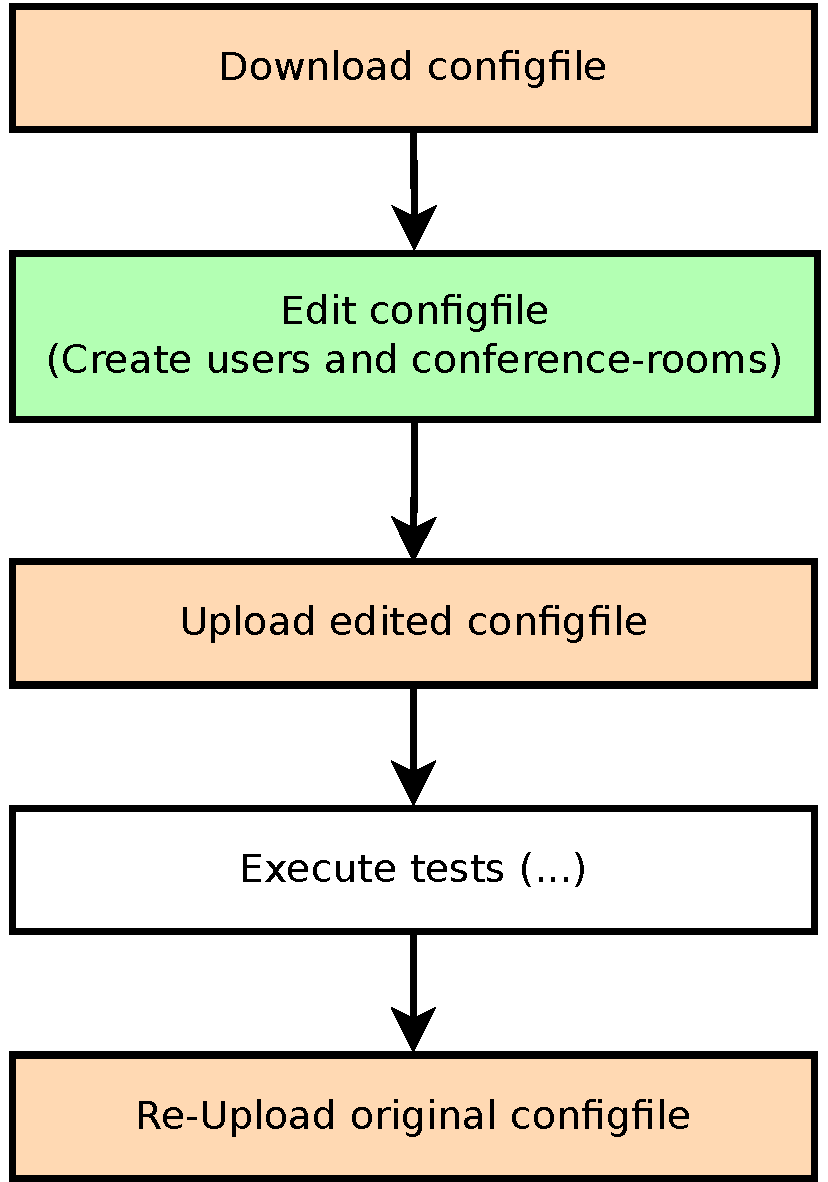
\includegraphics [width=7cm] {configuration-1}
\caption{Process of editing the Askozia-configuration file}
\end{figure}

%%%%%%%%%%%%%%%%%%%%%%%%%%%%%%%%%%%%%%%%%%%%%%%%%%%%%%
\subsection{Downloading/Uploading Configuration File}%
%%%%%%%%%%%%%%%%%%%%%%%%%%%%%%%%%%%%%%%%%%%%%%%%%%%%%%
For downloading the configuration file, it is necessary to send a HTML POST request to Askozia.
The useragent has to be authenticated as root and the content type must be ``multipart/form-data''.
For downloading the configuration file, the parameter ``Download'' has to be set.

\newpage In the performance test script, the following perl code is used to send this POST request:
\begin{lstlisting}[breaklines=true,label=code:config-post-request-download,caption={POST request for downloading the configuration file} ]
use HTTP::Request::Common;
use LWP;
my $ua = new LWP::UserAgent;
$ua->credentials ("$ask_ip:$ask_port",
	$ask_realm, "$ask_user" => "$ask_pw");
my $res = $ua->request (POST
	"http://$ask_ip:$ask_port/$ask_conf_page",
	"Content-Type" => "multipart/form-data",
	Content => [ Download => "1"]);
\end{lstlisting}

After executing this request, the following dataflow is to be expected:
\begin{figure} [h!]
\centering
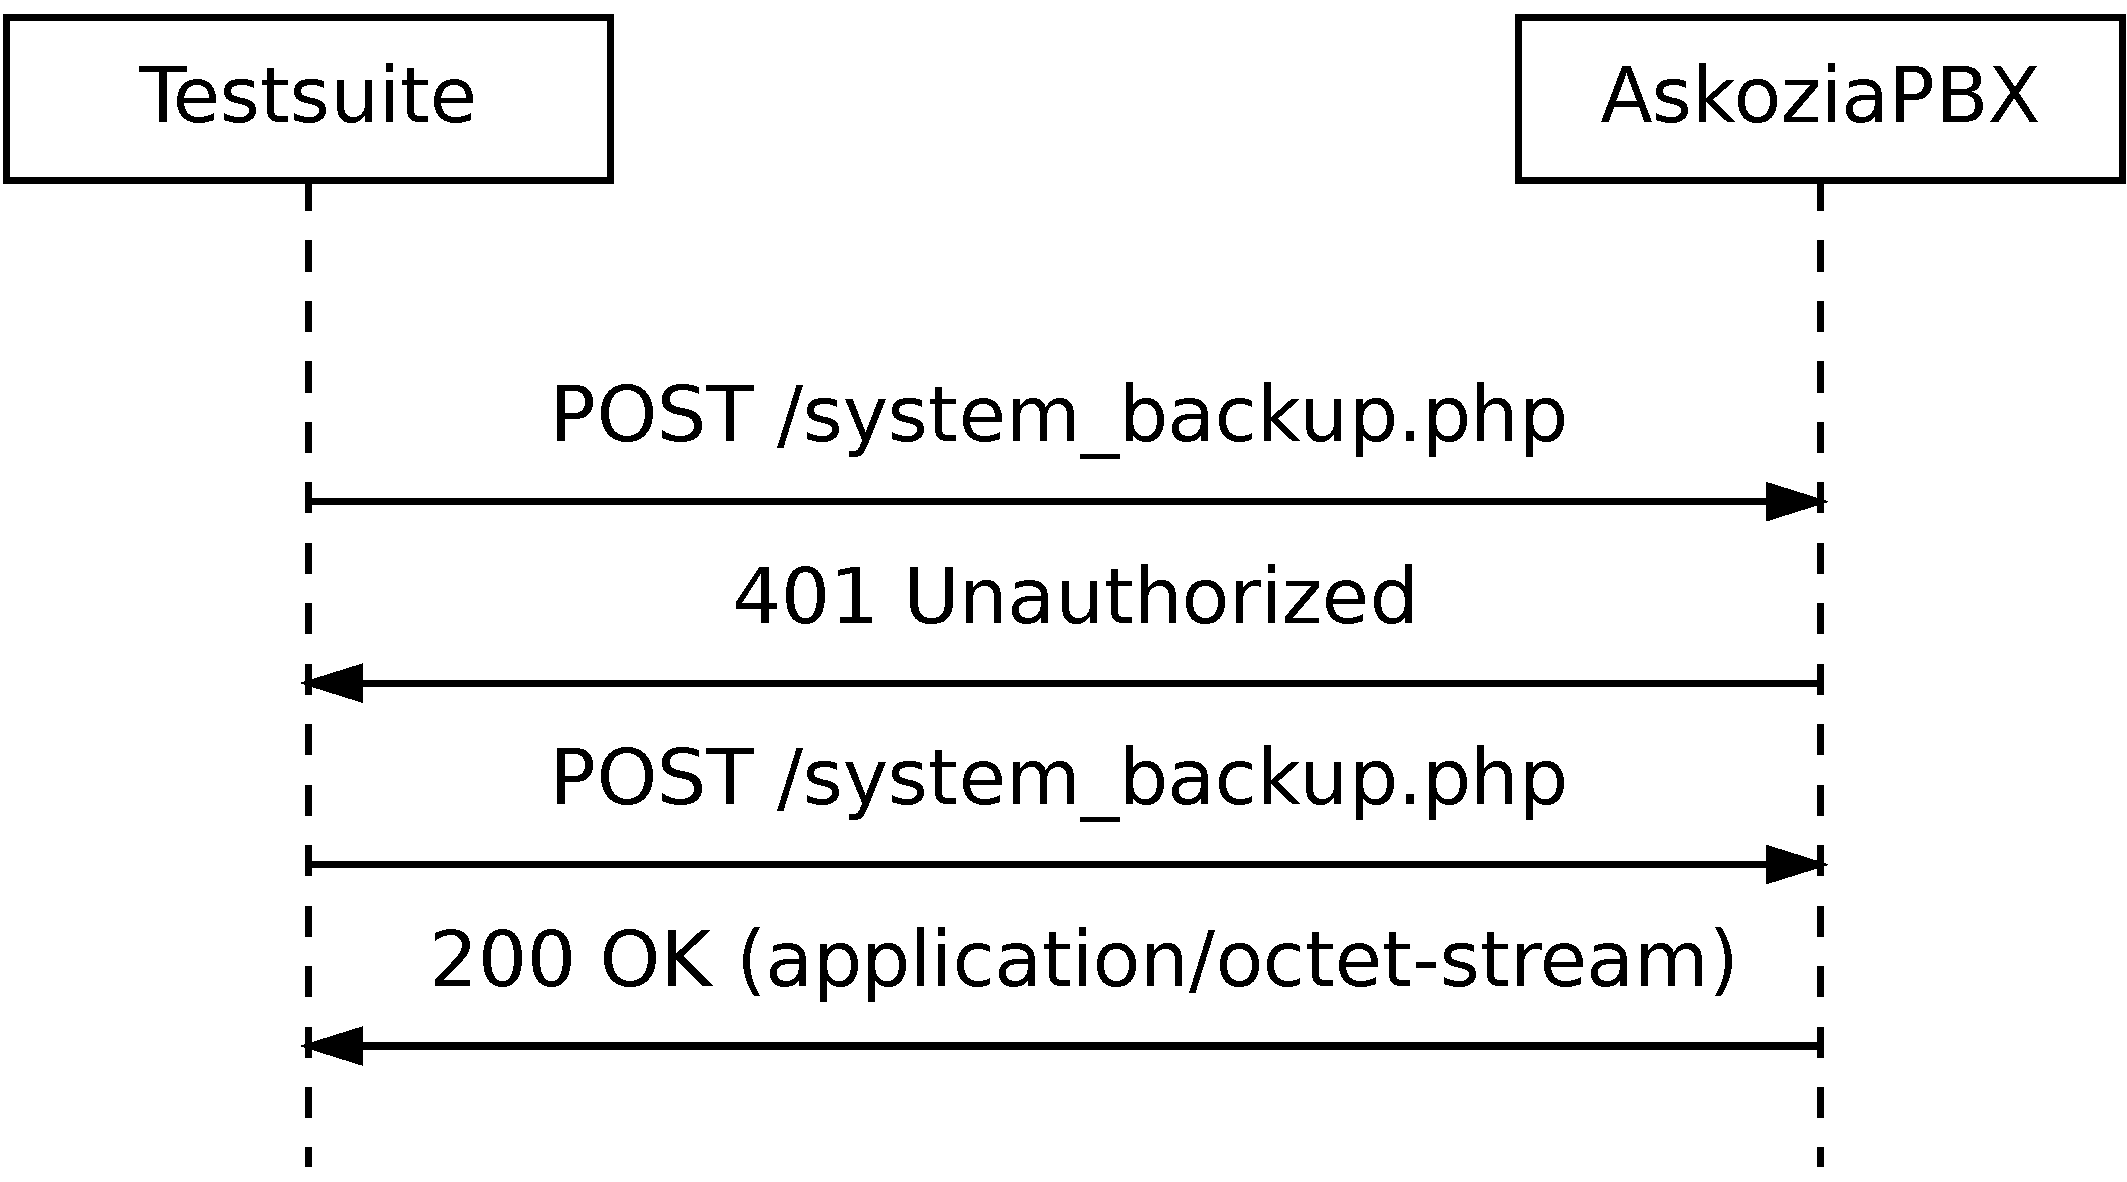
\includegraphics [width=11cm] {configuration-2}
\caption {Dataflow of configuration file download}
\end{figure}

The \texttt{200 OK} message sent by Askozia includes the configuration file in XML format. The XML file is saved with its original name
in the \texttt{./results/<testname>/} directory. Then, it is opened for reading to add the needed users and conference rooms
(see the next sections). When finished, the edited configuration file is saved with the original named followed by an \texttt{\_edited}
string. This edited configuration file is now uploaded to the AskoziaPBX as follows: \newpage

\begin{figure} [htbp]
\centering
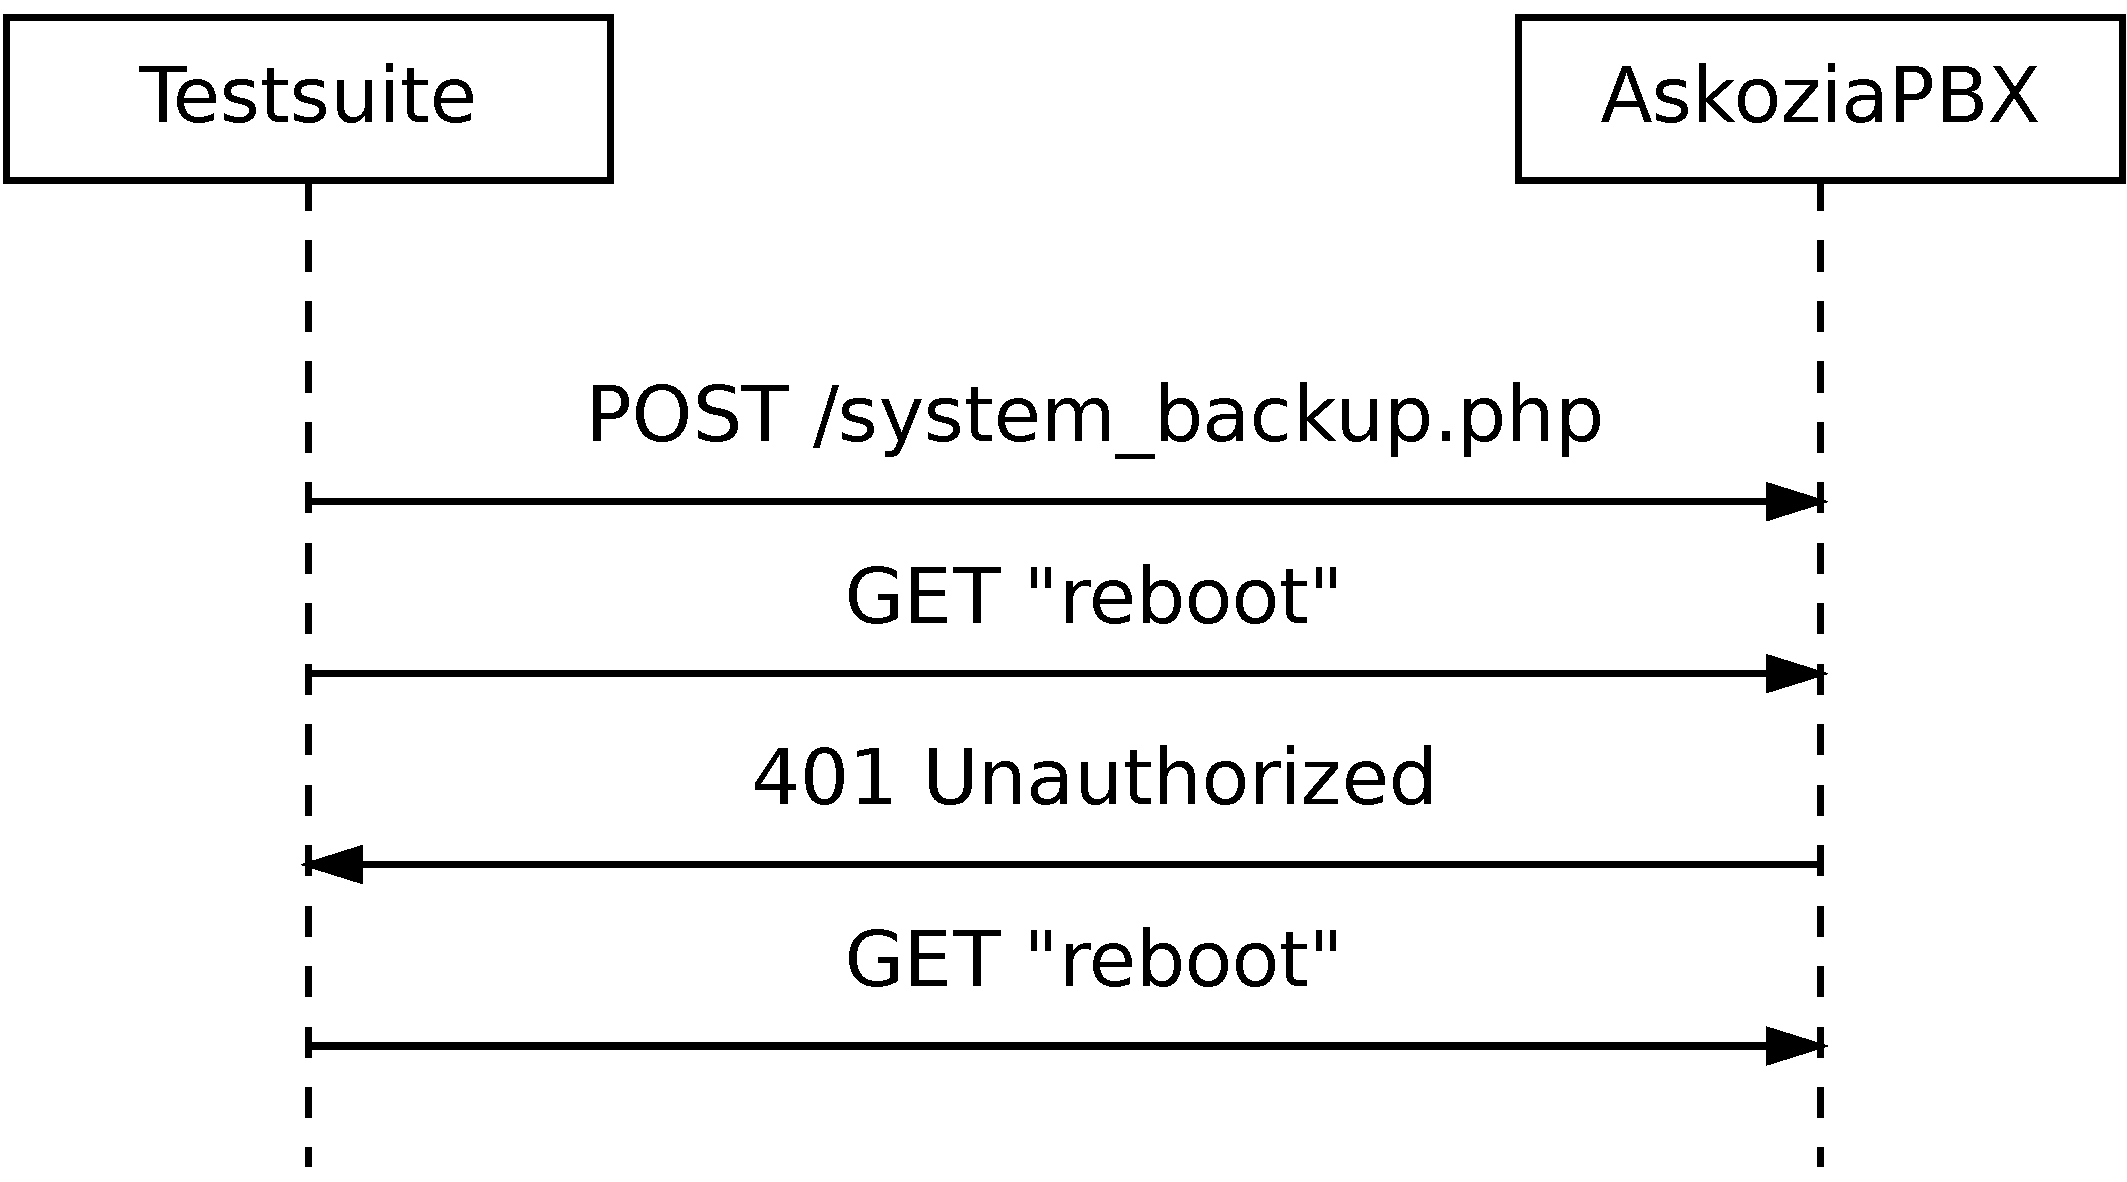
\includegraphics [width=11cm] {configuration-3}
\caption {Dataflow of configuration file upload}
\end{figure}

This dataflow is created by the following perl listing (\texttt{\$ua} and \texttt{\$res} are the existing variables declared and defined above):

\begin{lstlisting}[breaklines=true,label=code:config-post-request-upload,caption={POST request for uploading configuration file} ]
$res = $ua->request (POST
    "http://$ask_ip:$ask_port/$ask_conf_page",
	"Content-Type" => "multipart/form-data",
    Content => [ Restore => "1",
    conffile => [ $xml_configfile."_edited" ] ]);
\end{lstlisting}

After uploading the configuration file, the AskoziaPBX is rebooted.
This happenes automatically, but in this case, it is forced by an extra command sent as a GET request by using the webbased shell feature.
This manually forced reboot allows the script to ping Askozia and detect when it has finished rebooting.
Furthermore, it is now possible to wait some time (specified by using the \texttt{-{}-reboot-time} parameter)
to make sure that the PBX has enough time to start all services etc. after the reboot.
\begin{lstlisting}[breaklines=true,label=code:config-reboot,caption={Executing Askozia reboot} ]
my $ua = new LWP::UserAgent;
$ua->credentials ("$ask_ip:$ask_port",
    $ask_realm,	"$ask_user" => "$ask_pw");
$res = $ua->request (GET "http://$ask_ip:$ask_port/
    cgi-bin/ajax.cgi?exec_shell=reboot");
\end{lstlisting}


%%%%%%%%%%%%%%%%%%%
\subsection{Users}%
%%%%%%%%%%%%%%%%%%%
To execute the tests, it is necessary to add some test users to the AskoziaPBX installation.
The number of users depends on the parameters that were passed to the script when launching.
Here is a table of required users, the highest count will be added:

\begin{tabular}{|p{2cm}|p{12cm}|} \hline
	\textsc{Test type} & \textsc{Required users} \\ \hline \hline
	two-way & \texttt{= 2 * 2way-calls} (User A and B for each call) \\
	conf room & \texttt{= conf-calls-room * conf-rooms-room} \newline (``conf-calls'' users per ``conf-rooms'' conference rooms) \\
	conf call & \texttt{= conf-calls-call * conf-rooms-call} \newline (``conf-calls'' users per ``conf-rooms'' conference rooms) \\
	\hline
\end{tabular}

The script downloads the complete Askozia configuration file and searches for the end of the \texttt{sip} paragraph
Then, it adds its generated users. It is not checked whether the added phones already exist.
The template for adding users looks as follows, where \texttt{\_userno\_} is replaced by a three-digit integer that is incremented with each user:
\begin{lstlisting}[breaklines=true,label=code:config-user-template,caption={User template} ]
<phone>
<extension>_userno_</extension>
<callerid>Testuser _userno_</callerid>
<manualattributes>cXVhbGlmeT1ubw==</manualattributes>
<codec>alaw</codec>
<secret>_userno_</secret>
<uniqid>SIP-PHONE-_userno_</uniqid>
<language>en-us</language>
<ringlength>indefinitely</ringlength>
<natmode>yes</natmode>
<dtmfmode>auto</dtmfmode>
</phone>
\end{lstlisting}

%%%%%%%%%%%%%%%%%%%%%%%%%%%%%%
\subsection{Conference Rooms}%
%%%%%%%%%%%%%%%%%%%%%%%%%%%%%%
Just like the users, the needed conference rooms have to be added too.
The script searches for the end of the \texttt{conferencing} paragraph and adds its generated rooms.
The template looks as follows, where \texttt{\_roomno\_} is replaced by an integer that is incremented with each room:
\begin{lstlisting}[breaklines=true,label=code:config-room-template,caption={Conference room template} ]
<room>
<number>_roomno_</number>
<name>Default Conference</name>
<uniqid>CONFERENCE-ROOM-_roomno_</uniqid>
</room>
\end{lstlisting}

Conference rooms start with number 2000 (can be changed).
So, for a conference test that needs ten conference rooms, rooms from 2000 to 2009 are created.

\section{Two-Party Tests}
\label{sec:two-party}

Two-Party tests are the normal telephone calls between two participants.
User A calls another user (perhaps User B) who has to be registered, makes a phone call and hangs up.

As a \texttt{sip} dialog, the scenario looks as follows:
\begin{figure} [!ht]
\centering
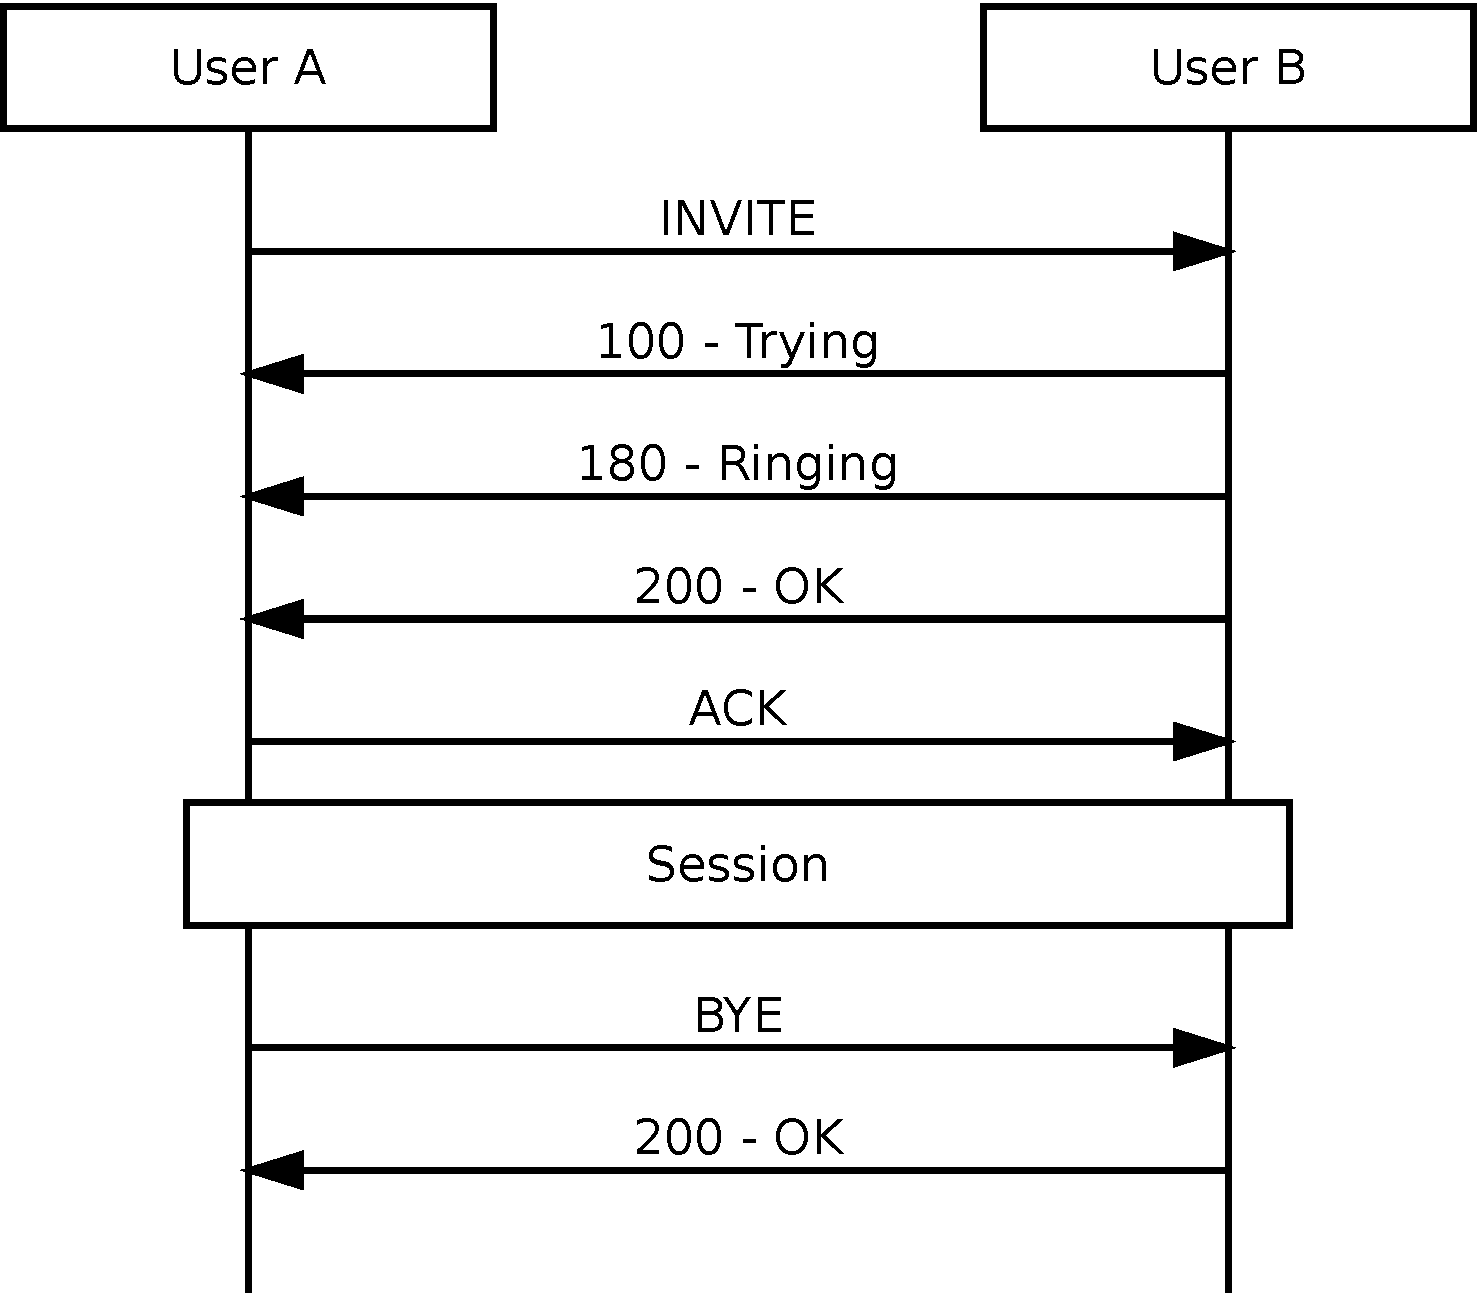
\includegraphics [width=10cm] {twoway-1}
\caption{SIP dialog of a two-party call}
\end{figure}
The original XML scenarios for sipp used to implement this are available in the appendix. \newpage

\begin{figure} [!ht]
\centering
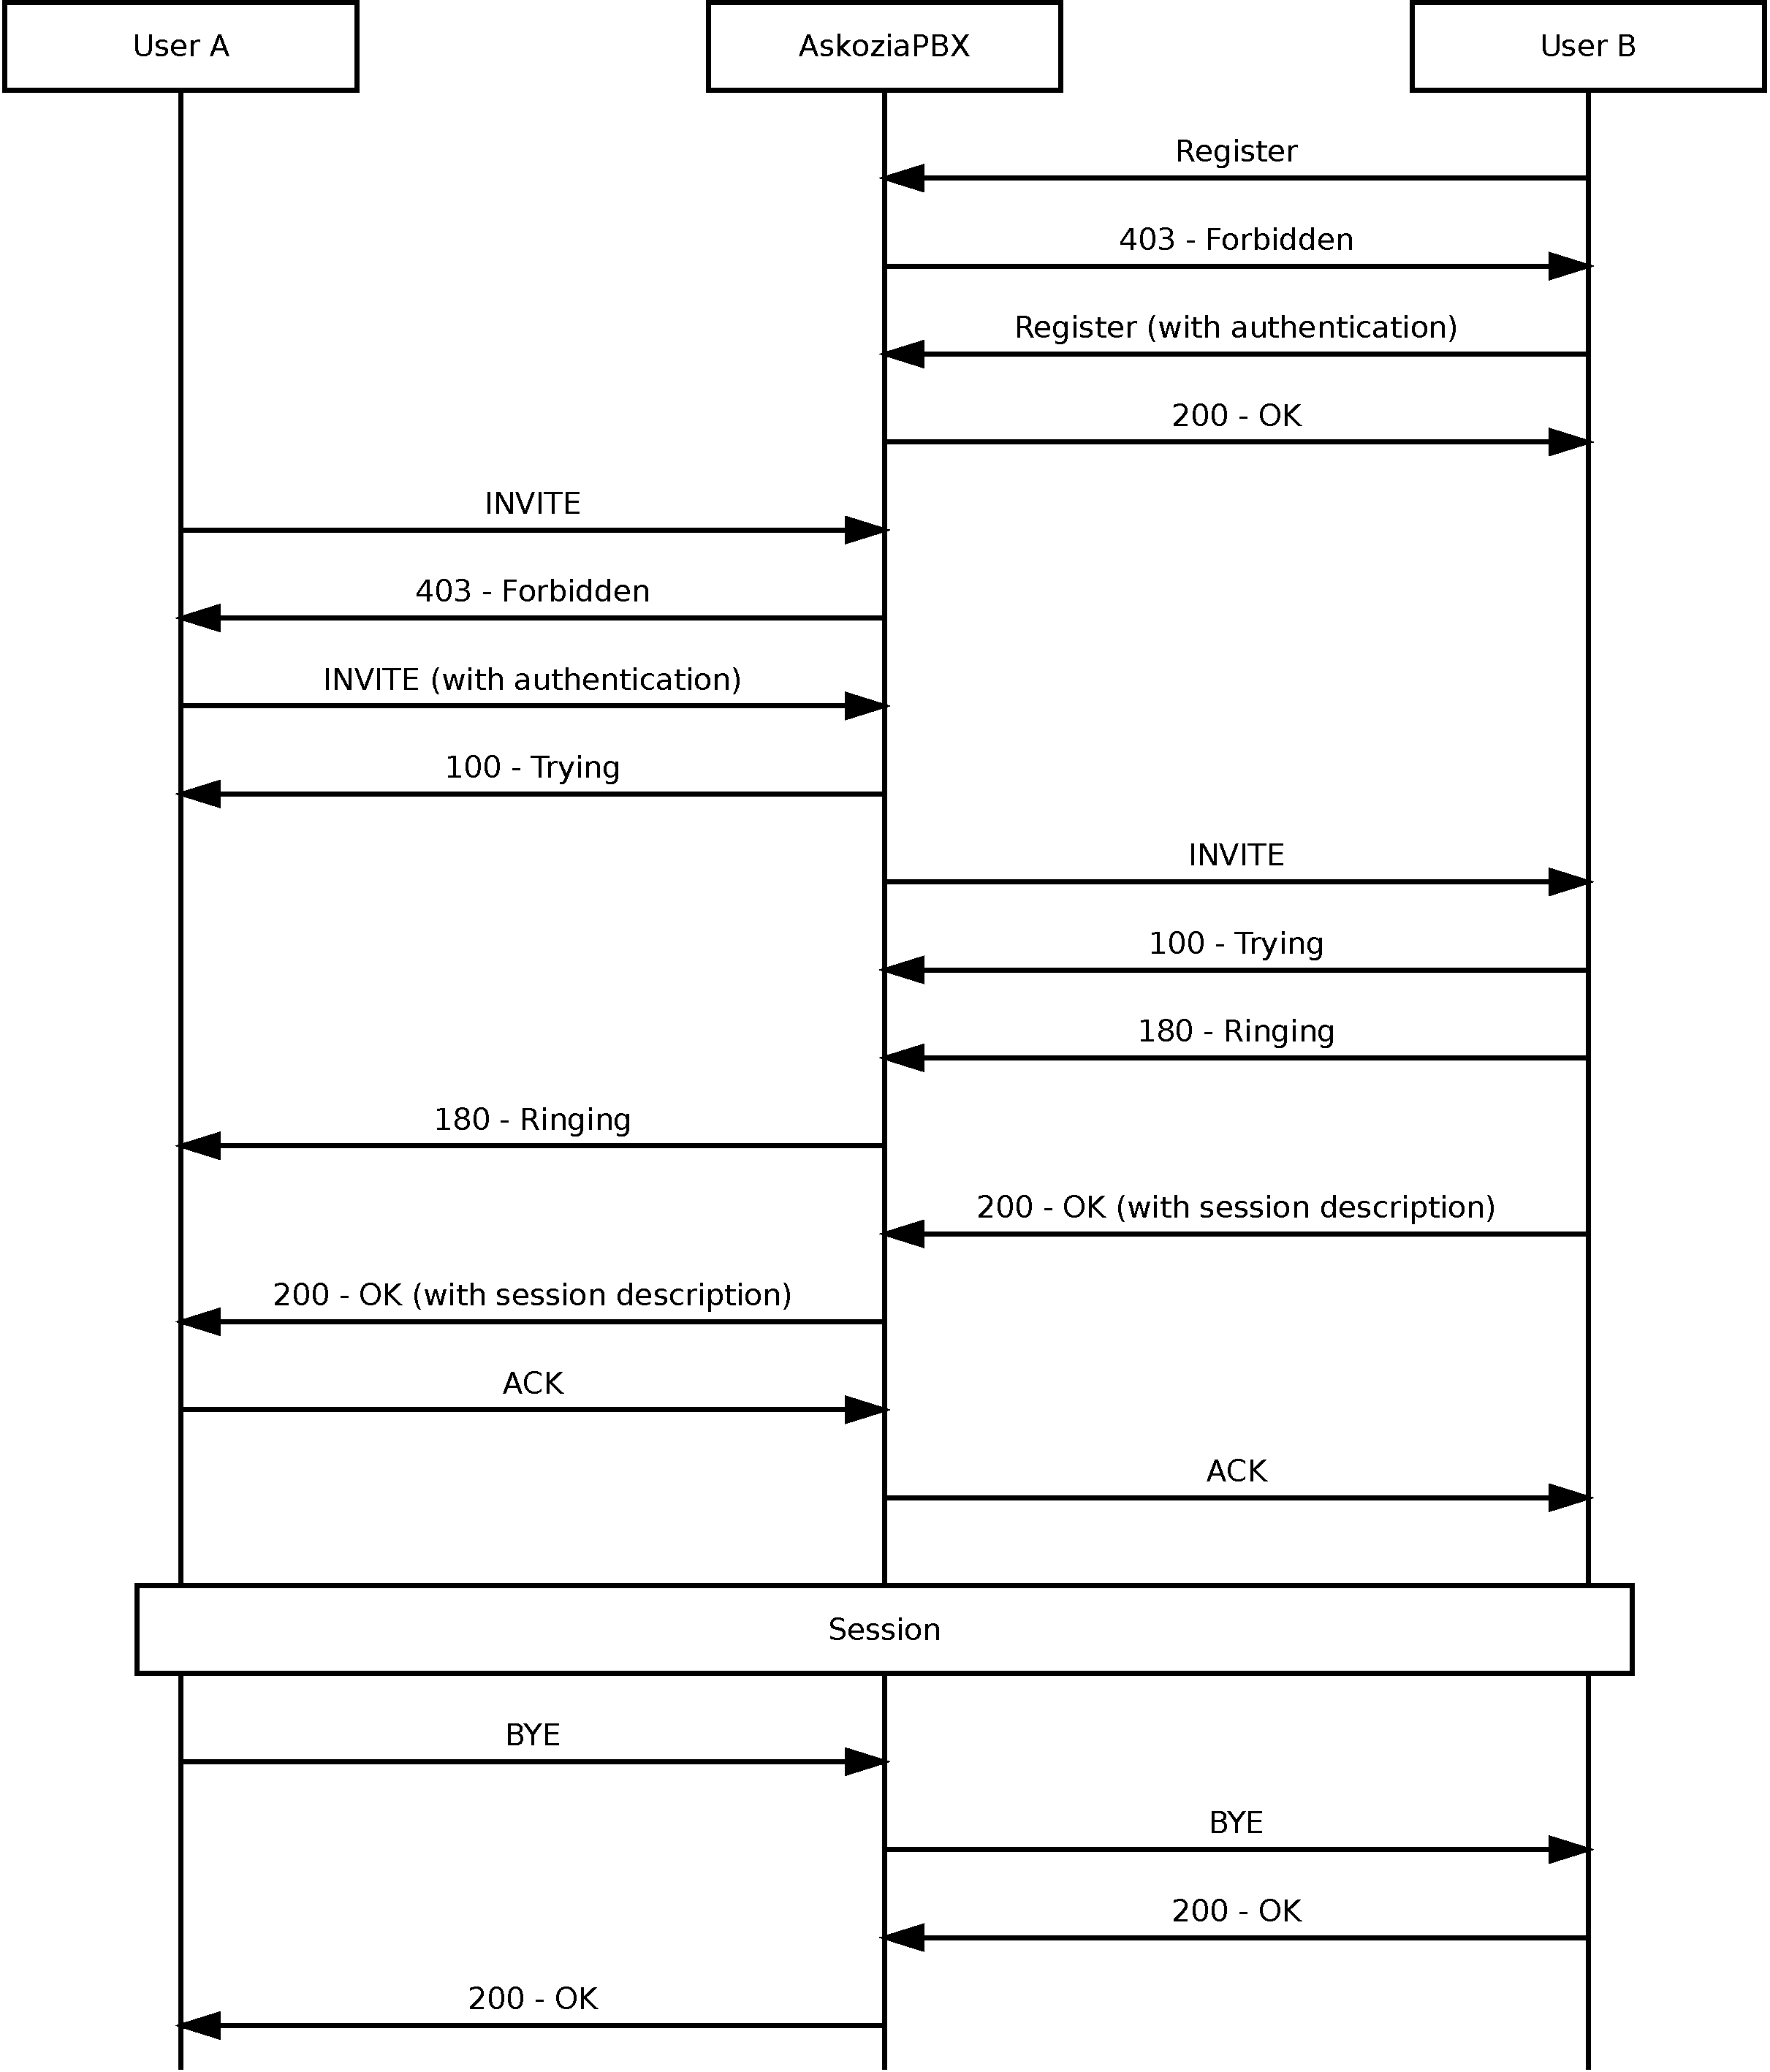
\includegraphics [width=15cm] {twoway-2}
\caption{Dialog of a two-party call}
\end{figure}

The next diagramm shows the process of a complete two-party test: \newpage
\begin{figure} [!ht]
\centering
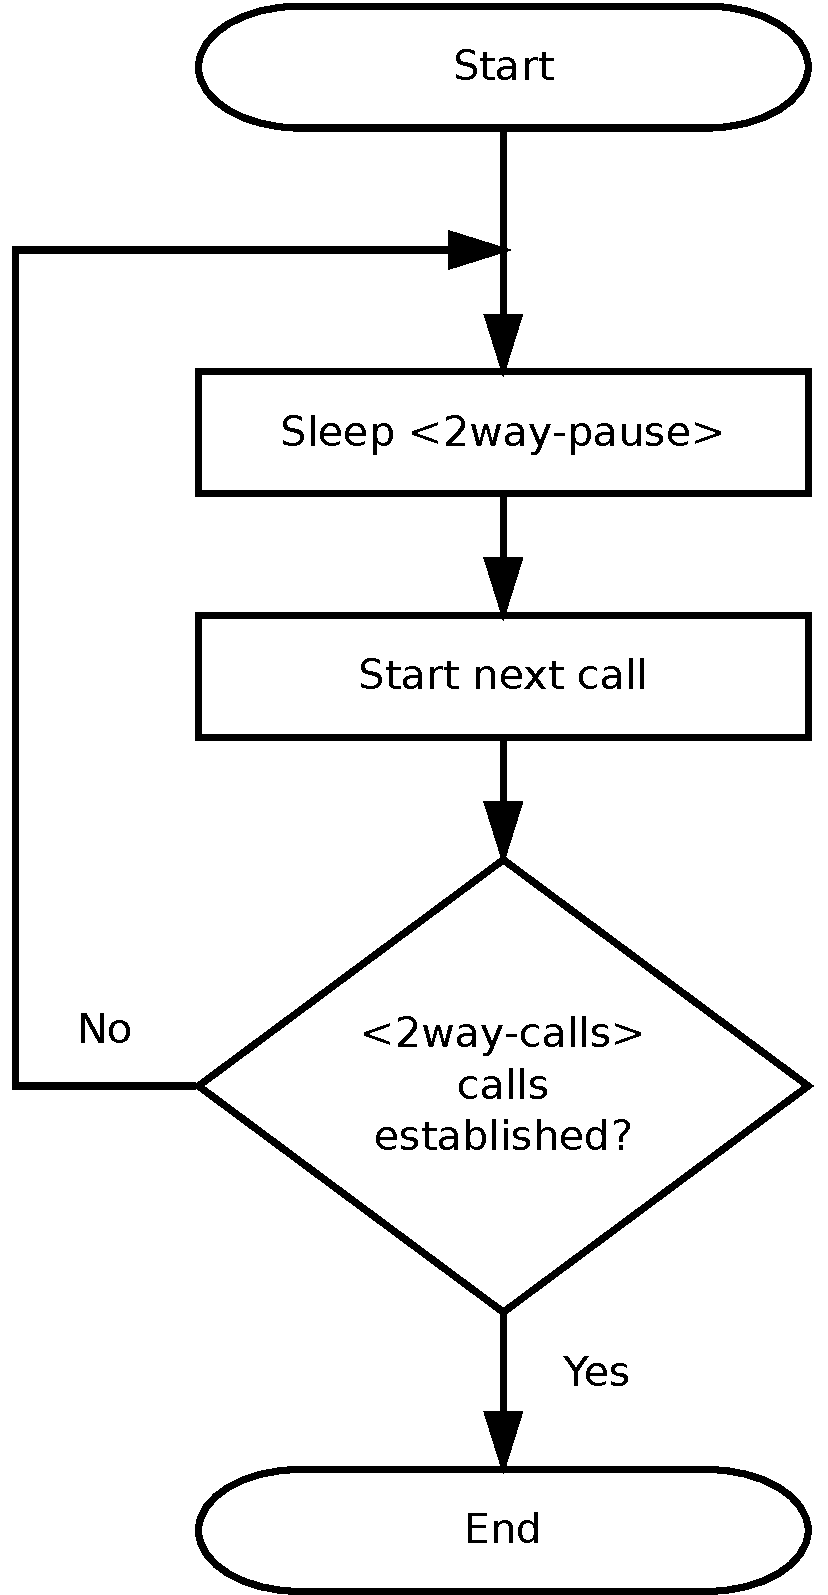
\includegraphics [width=6cm] {twoway-3}
\caption{Complete two-party test}
\end{figure}

The number of calls is increased step-by-step. After every call, the script waits for the specified pause
time to record the CPU load values. For executing two-party calls, the following sipp commands used.
You can inform yourself about the used parameters by reading the sipp manpage (the appendix contains the sipp manpage).
\begin{lstlisting}[breaklines=true,label=code:twoway-invite,caption={sipp command for inviting User B} ]
REGISTER Command:
$sipp -aa -inf '$users_twoway_file' -m $current_call -i $local_ip
  -p $sip_dst_port -mp $rtp_dst_port -sf '$reg_scen' $ask_ip 2>&1

ACCEPT Command:
sipp -aa -inf '$users_twoway_file' -m $current_call -i $local_ip
  -p $sip_dst_port -mp $rtp_dst_port -sf '$acc_scen' -bg $ask_ip 2>&1 &

INVITE Command:
sipp -aa -inf '$users_twoway_file' -m $current_call -i $local_ip
  -p $sip_src_port -mp $rtp_src_port -sf '$inv_scen' $ask_ip 2>&1

De-REGISTER Command:
sipp -aa -inf '$users_twoway_file' -m $current_call -i $local_ip
  -p $sip_dst_port -mp $rtp_dst_port -sf '$der_scen' $ask_ip 2>&1
\end{lstlisting}


\section{Maximum Three-Way Conference Rooms Tests}
\label{sec:conf-rooms-test}

The conference rooms test was developed primarily for executing three-way conferences.
Basically, there is a conference with three participants started. After that, there is another conference
with three participants started until the maximum number of conferences is reached:

\begin{figure} [!ht]
\centering
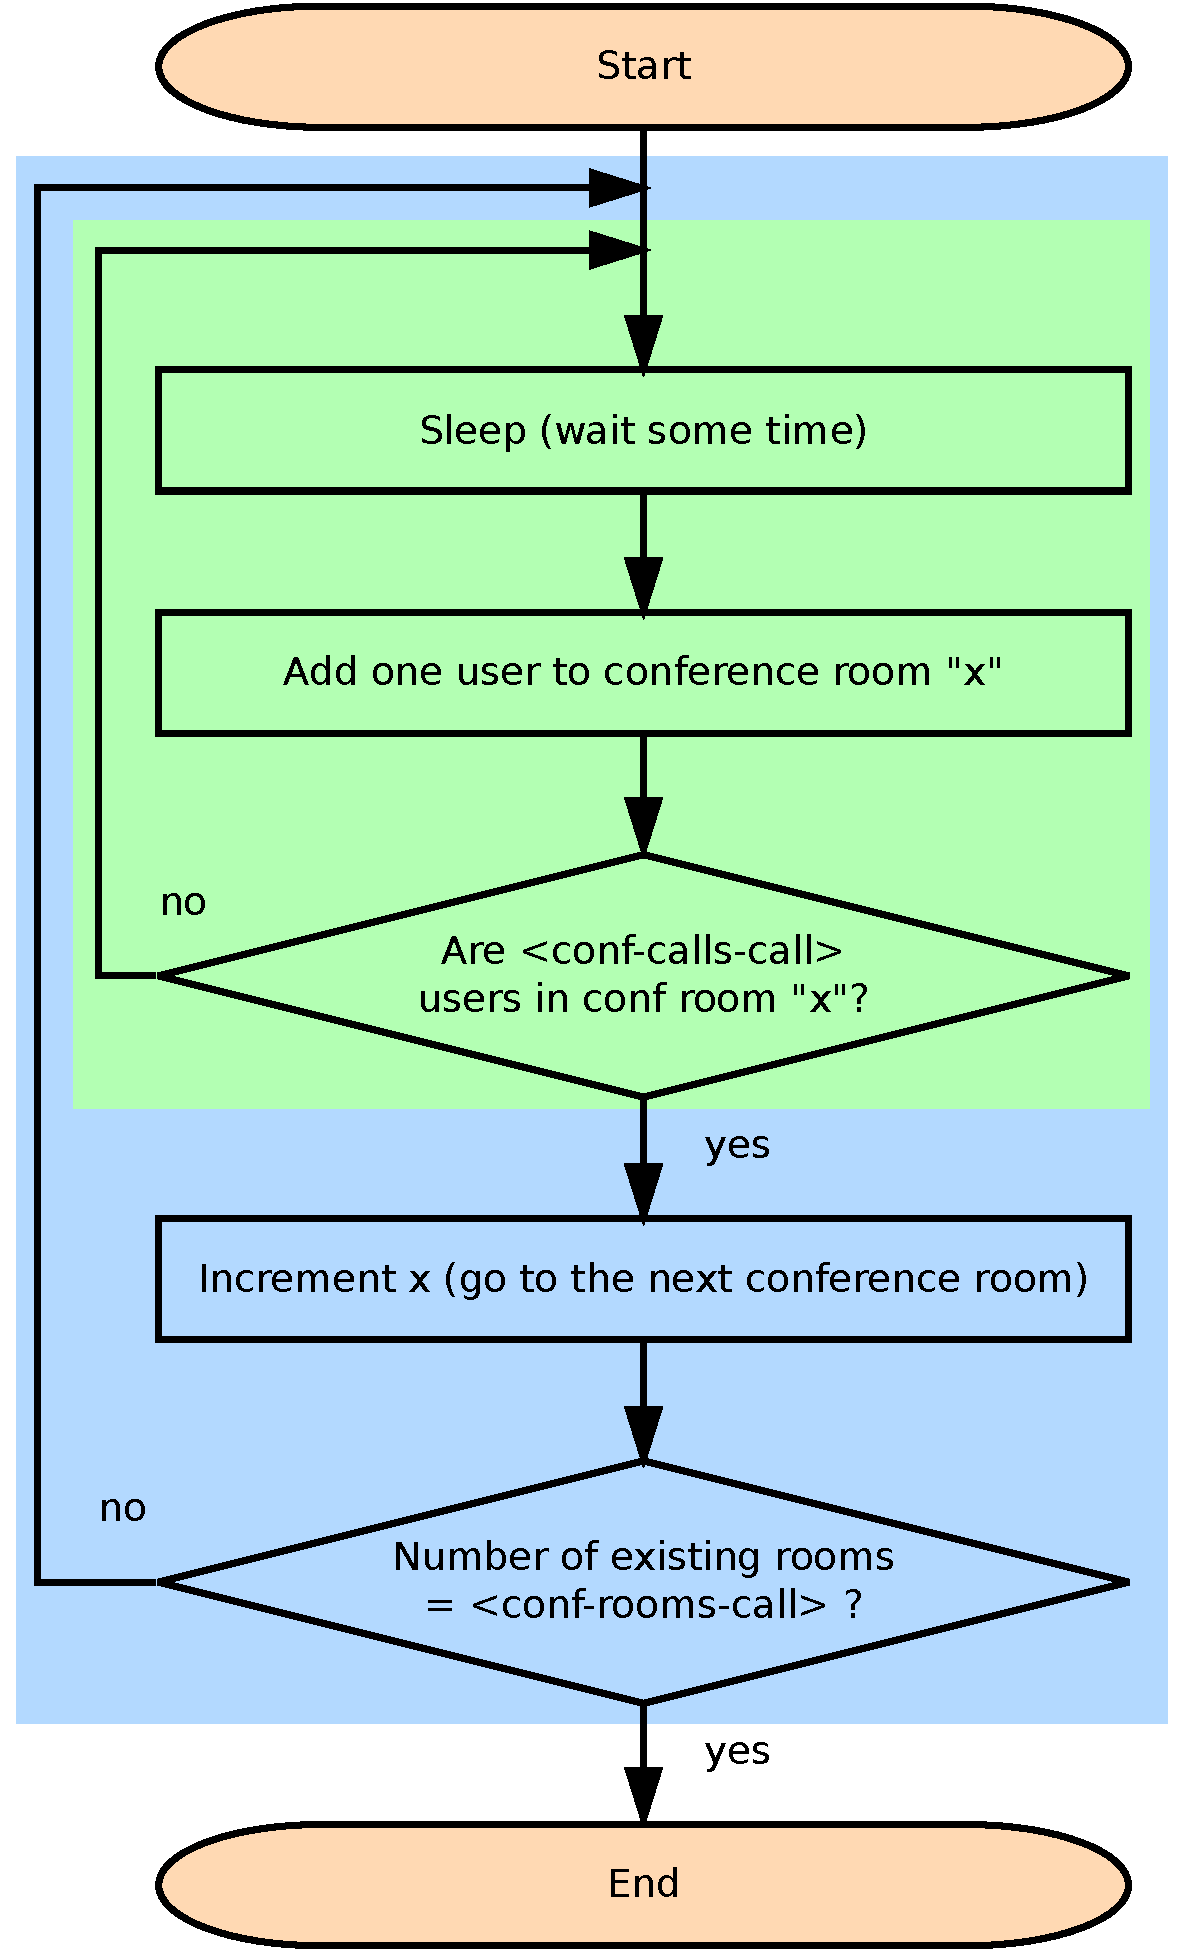
\includegraphics [width=8cm] {conf-rooms-test-1}
\caption{Process of conference rooms tests}
\end{figure}

For a conf call test with three participants and four conference rooms, the test would work like this: \newpage
\begin{figure} [!ht]
\centering
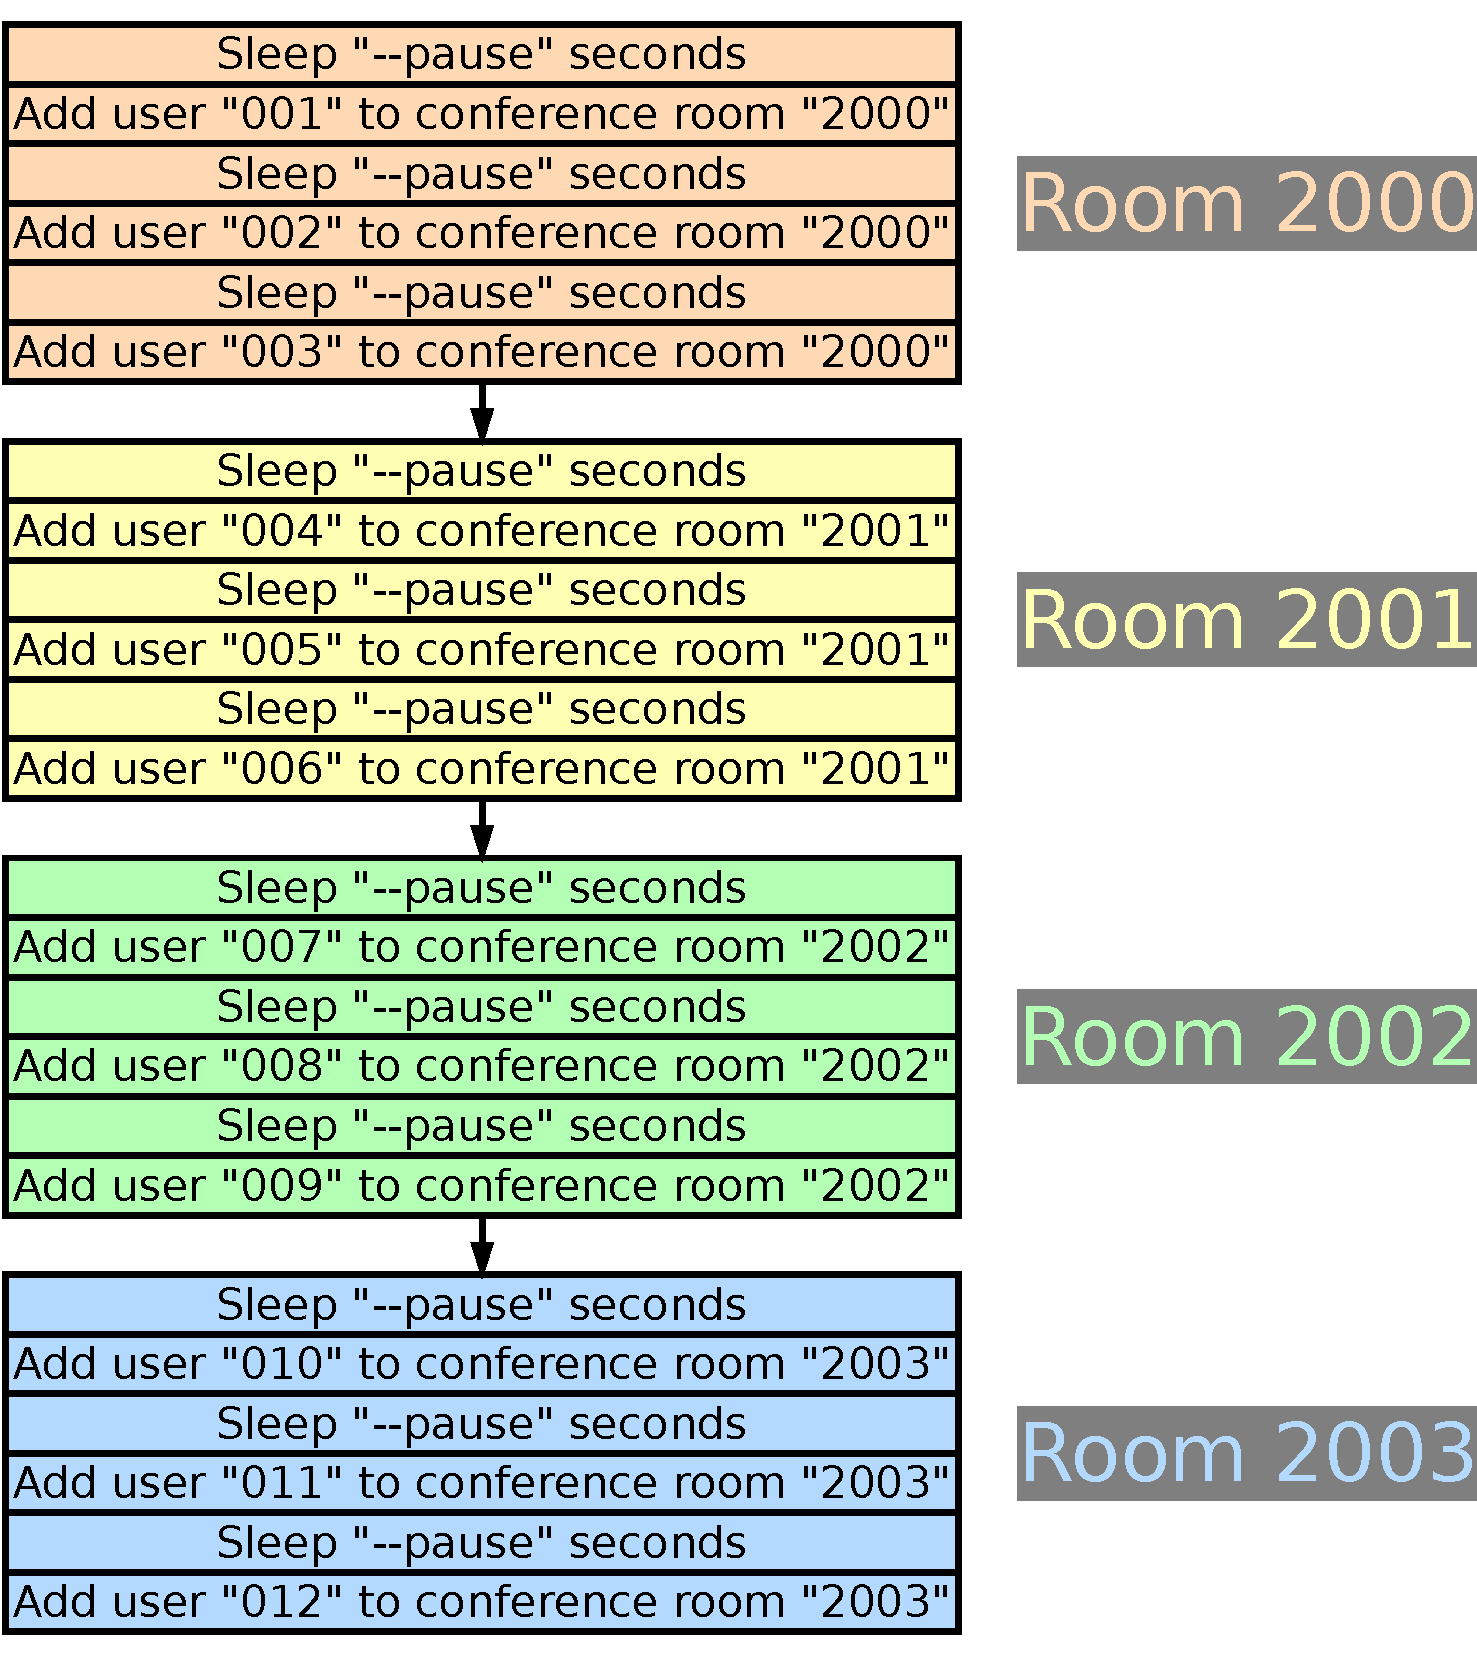
\includegraphics [width=8cm] {conf-rooms-test-2}
\caption{Conference rooms test example}
\end{figure}

This is implemented by using the sipp functionalities \texttt{call rates} (parameter -r)  and \texttt{rate period} (parameter -rp):
\begin{lstlisting}[breaklines=true,label=code:conf-call-invite,caption={sipp command for starting conf call tests} ]
sipp -aa -r 1
    -i $local_ip
    -rp 60s 
    -inf 'Users_conf-rooms.csv'
    -m $current_users
    -p 5061
    -mp 6020
    -sf 'Invite.xml'
    $ask_ip 2>&1"
\end{lstlisting}

\texttt{-rp 60s} is the rate period in seconds; \texttt{-r 1 -rp 60s} means that 1 user is added
every 60 seconds. With this scenario, the following situation is simulated:

\begin{figure} [!ht]
\centering
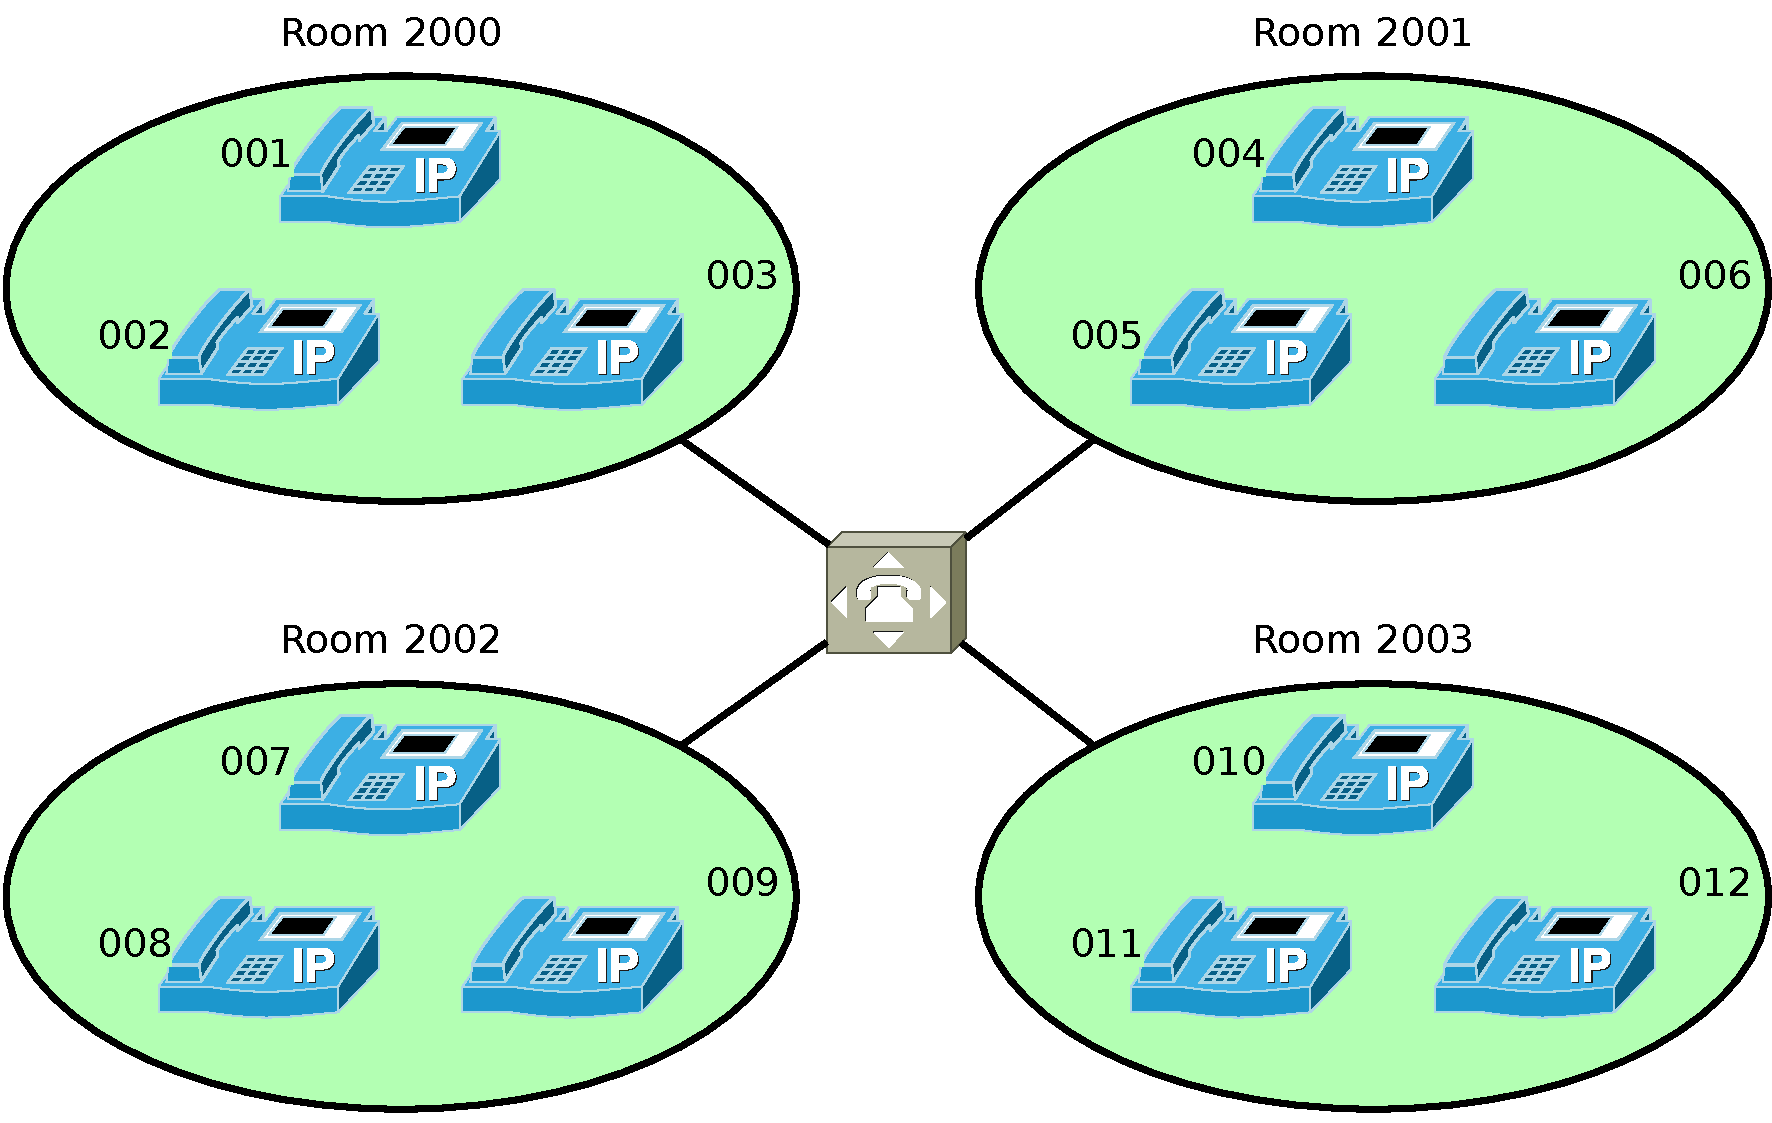
\includegraphics [width=10cm] {conf-rooms-test-3}
\caption {Conference rooms test illustration with 3 calls, 4 rooms}
\label {fig:conf-call-illustration}
\end{figure}


\section{Maximum Participants in a Single Conference Room Test}
\label{sec:conf-participants-test}

The conference participants test was developed primarily for simulating one conference room with any
number of participants. So, since the number of rooms is fixed, the number of calls has to be increased step-by-step:

\begin{figure} [!ht]
\centering
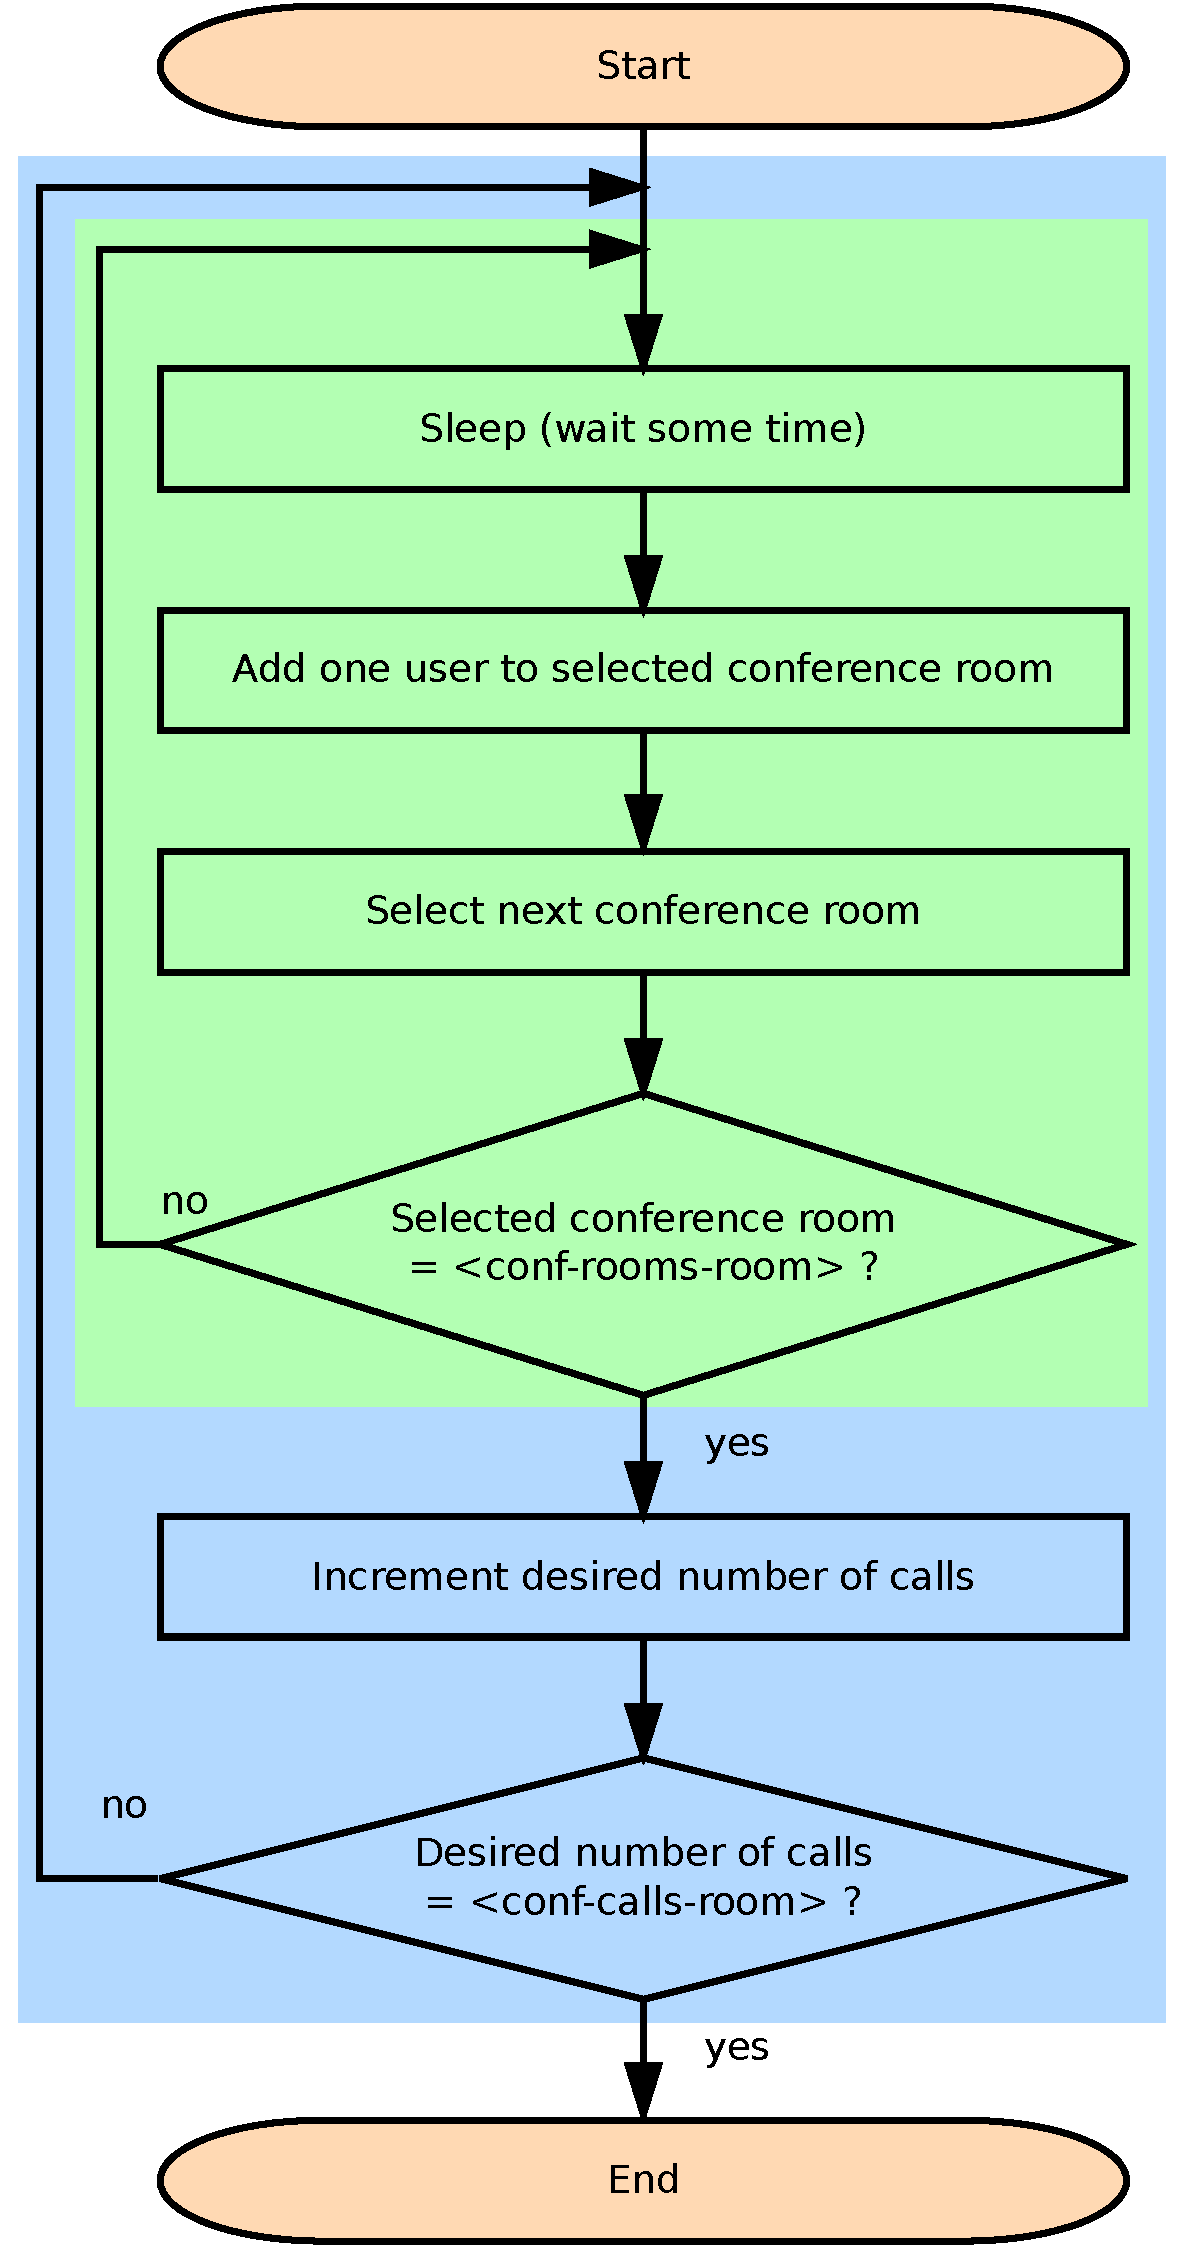
\includegraphics [width=8cm] {conf-participants-test-1}
\caption{Process of conference participants test}
\end{figure}

\newpage
For a conference participants test with five calls, the test would work like this: 
\begin{figure} [!ht]
\centering
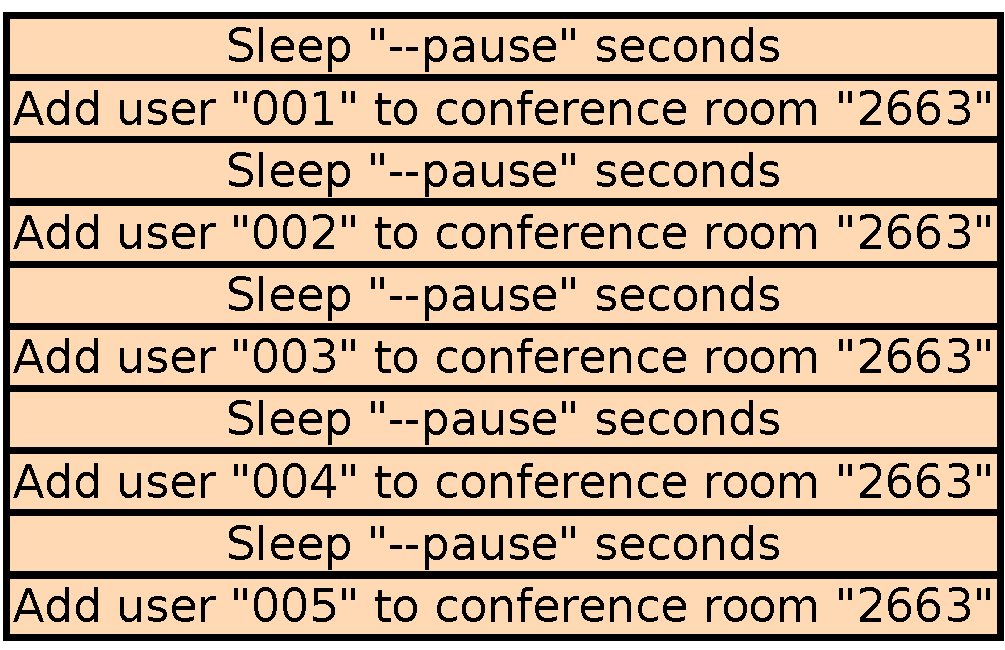
\includegraphics [width=8cm] {conf-participants-test-2}
\caption{Conference participants test example}
\end{figure}

The command for executing \texttt{sipp} looks as follows:

\begin{lstlisting}[breaklines=true,label=code:conf-room-invite,caption={sipp command for starting conference participants tests} ]
sipp -r 1 -aa
  -rp 60s
  -inf 'Users_conf-participants.csv'
  -m $current_users
  -i $local_ip
  -p 5061
  -mp 6020
  -sf 'Invite.xml'
  $ask_ip 2>&1"
\end{lstlisting}

\section{Watchdog Feature}
\label{sec:watchdog}

The watchdog feature is a component that stops testing after a defined time. It is necessary because the AskoziaPBX does not respond
any more if it reaches its limit. Is is implemented like that:

\begin{figure} [!ht]
\centering
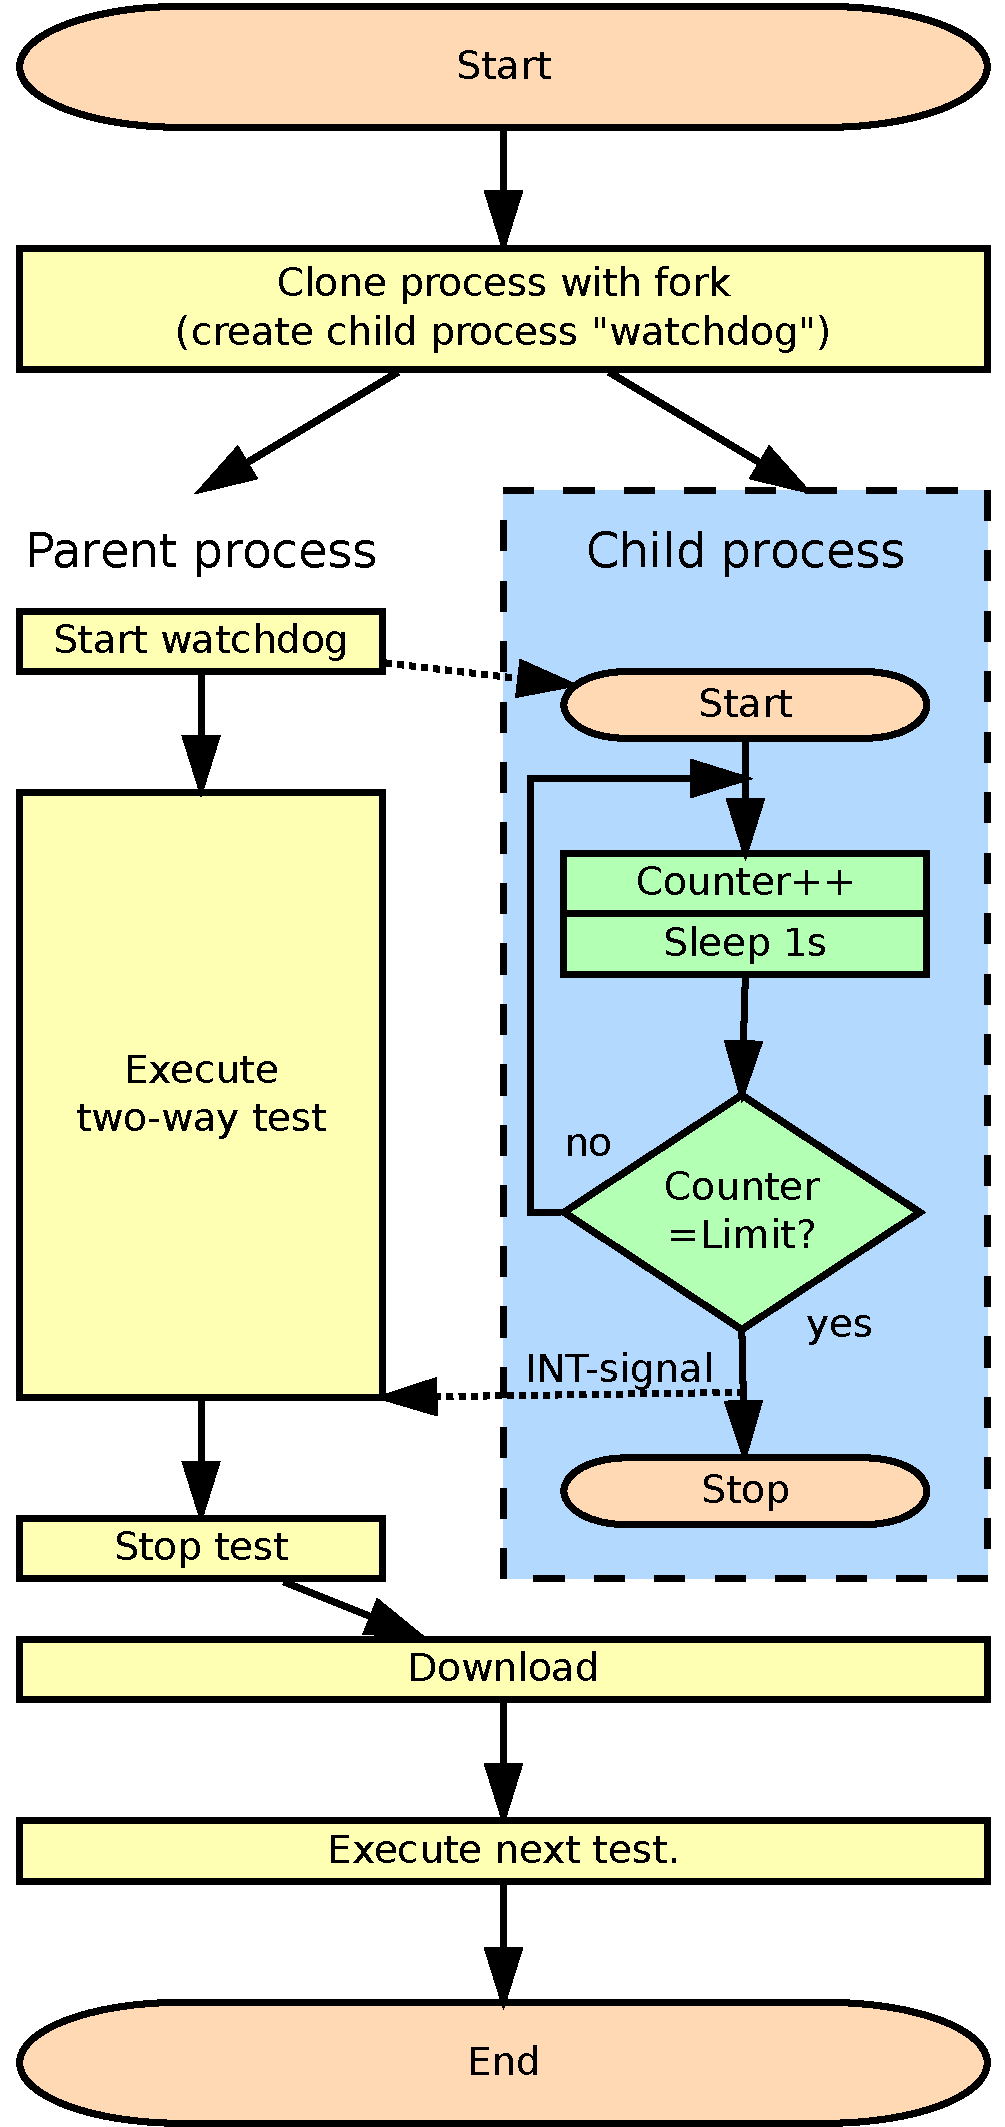
\includegraphics [width=8cm] {watchdog-1}
\caption{Basic watchdog process}
\label{fig:watchdog-basic-process}
\end{figure}

\newpage
Of course, it is not as easy as it is shown in figure~\ref{fig:watchdog-basic-process}. First of all,
there is only one watchdog process that is forked before beginning the tests.
This process is started and stopped multiple times (one time for every test type):

\begin{figure} [!ht]
\centering
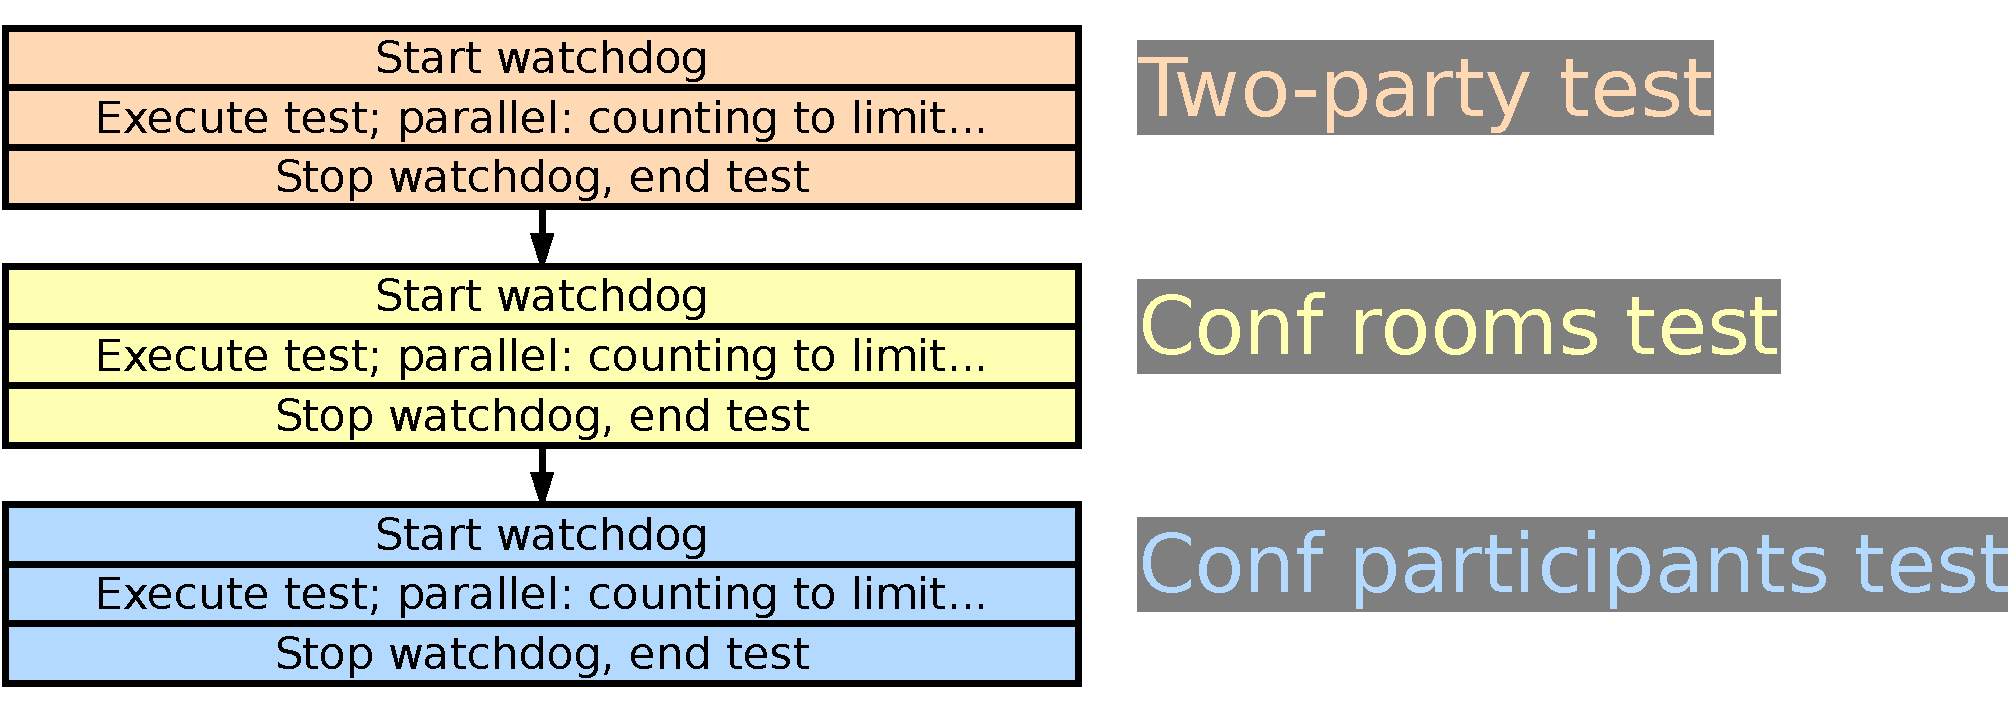
\includegraphics [width=14cm] {watchdog-2}
\caption{Starts and stops of watchdog}
\end{figure}

Let's sum up: Now there is a second process that is started before every test and stopped after every test.
At the end of all tests, it is killed. But there is still one problem: Because of the variable parameters,
the tests may have very different durations. So, it is necessary to tell the watchdog some settings of the test.
For this reason, there is an IPC (Interprocess Communication) existing. After forking the main process, there
is a pipe created to send messages from the parent (test) process to the child (watchdog). It can be treated
like a normal print device in perl, so it is possible to send messages like this:

\begin{lstlisting}[breaklines=true,label=code:watchdog-pipe,caption={Send messages to watchdog} ]
print $pipe $message;
\end{lstlisting}

It is possible to send to following commands to the watchdog. All commands have to end with a newline character
for flushing the pipe:

\begin{tabular}{|p{3.5cm}|p{10.5cm}|} \hline
\textsc{Testtype} & \textsc{Needed users} \\ \hline \hline
\texttt{set pause '3'}		& Set pause time to 3 seconds \newline (necessary for call duration calculation) \\
\texttt{set users '5'}		& Set number of users to 5 \newline (necessary for call duration calculation) \\
\texttt{start watchdog}		& Starts watchdog: Begin of incrementing counter per second \\
\texttt{stop watchdog}		& Stops watchdog (incrementing counter) \\
\texttt{Tests finished.}	& Terminates watchdog process. \\
\hline
\end{tabular}

After sending a command, the counter is reset to zero automatically (there is no provision for sending commands
to the watchdog while running a test). Sometimes, there were problems if two commands are sent in quick succession, 
so it is recommended to sleep one second between sending two commands.


\section{Recording CPU Load}
\label{sec:qstat}

Recording the CPU load is executed by a self-programmed tool of Michael Iedema (michael\@askozia.com). Its name is
\texttt{qstat} and is available by pressing the \texttt{ESC} key somewhere on the Askozia webpage. Then, in the
``Beta Features'' tab, there is a link referencing to \texttt{debug\_qstat.php}:

\begin{figure} [!ht]
\centering
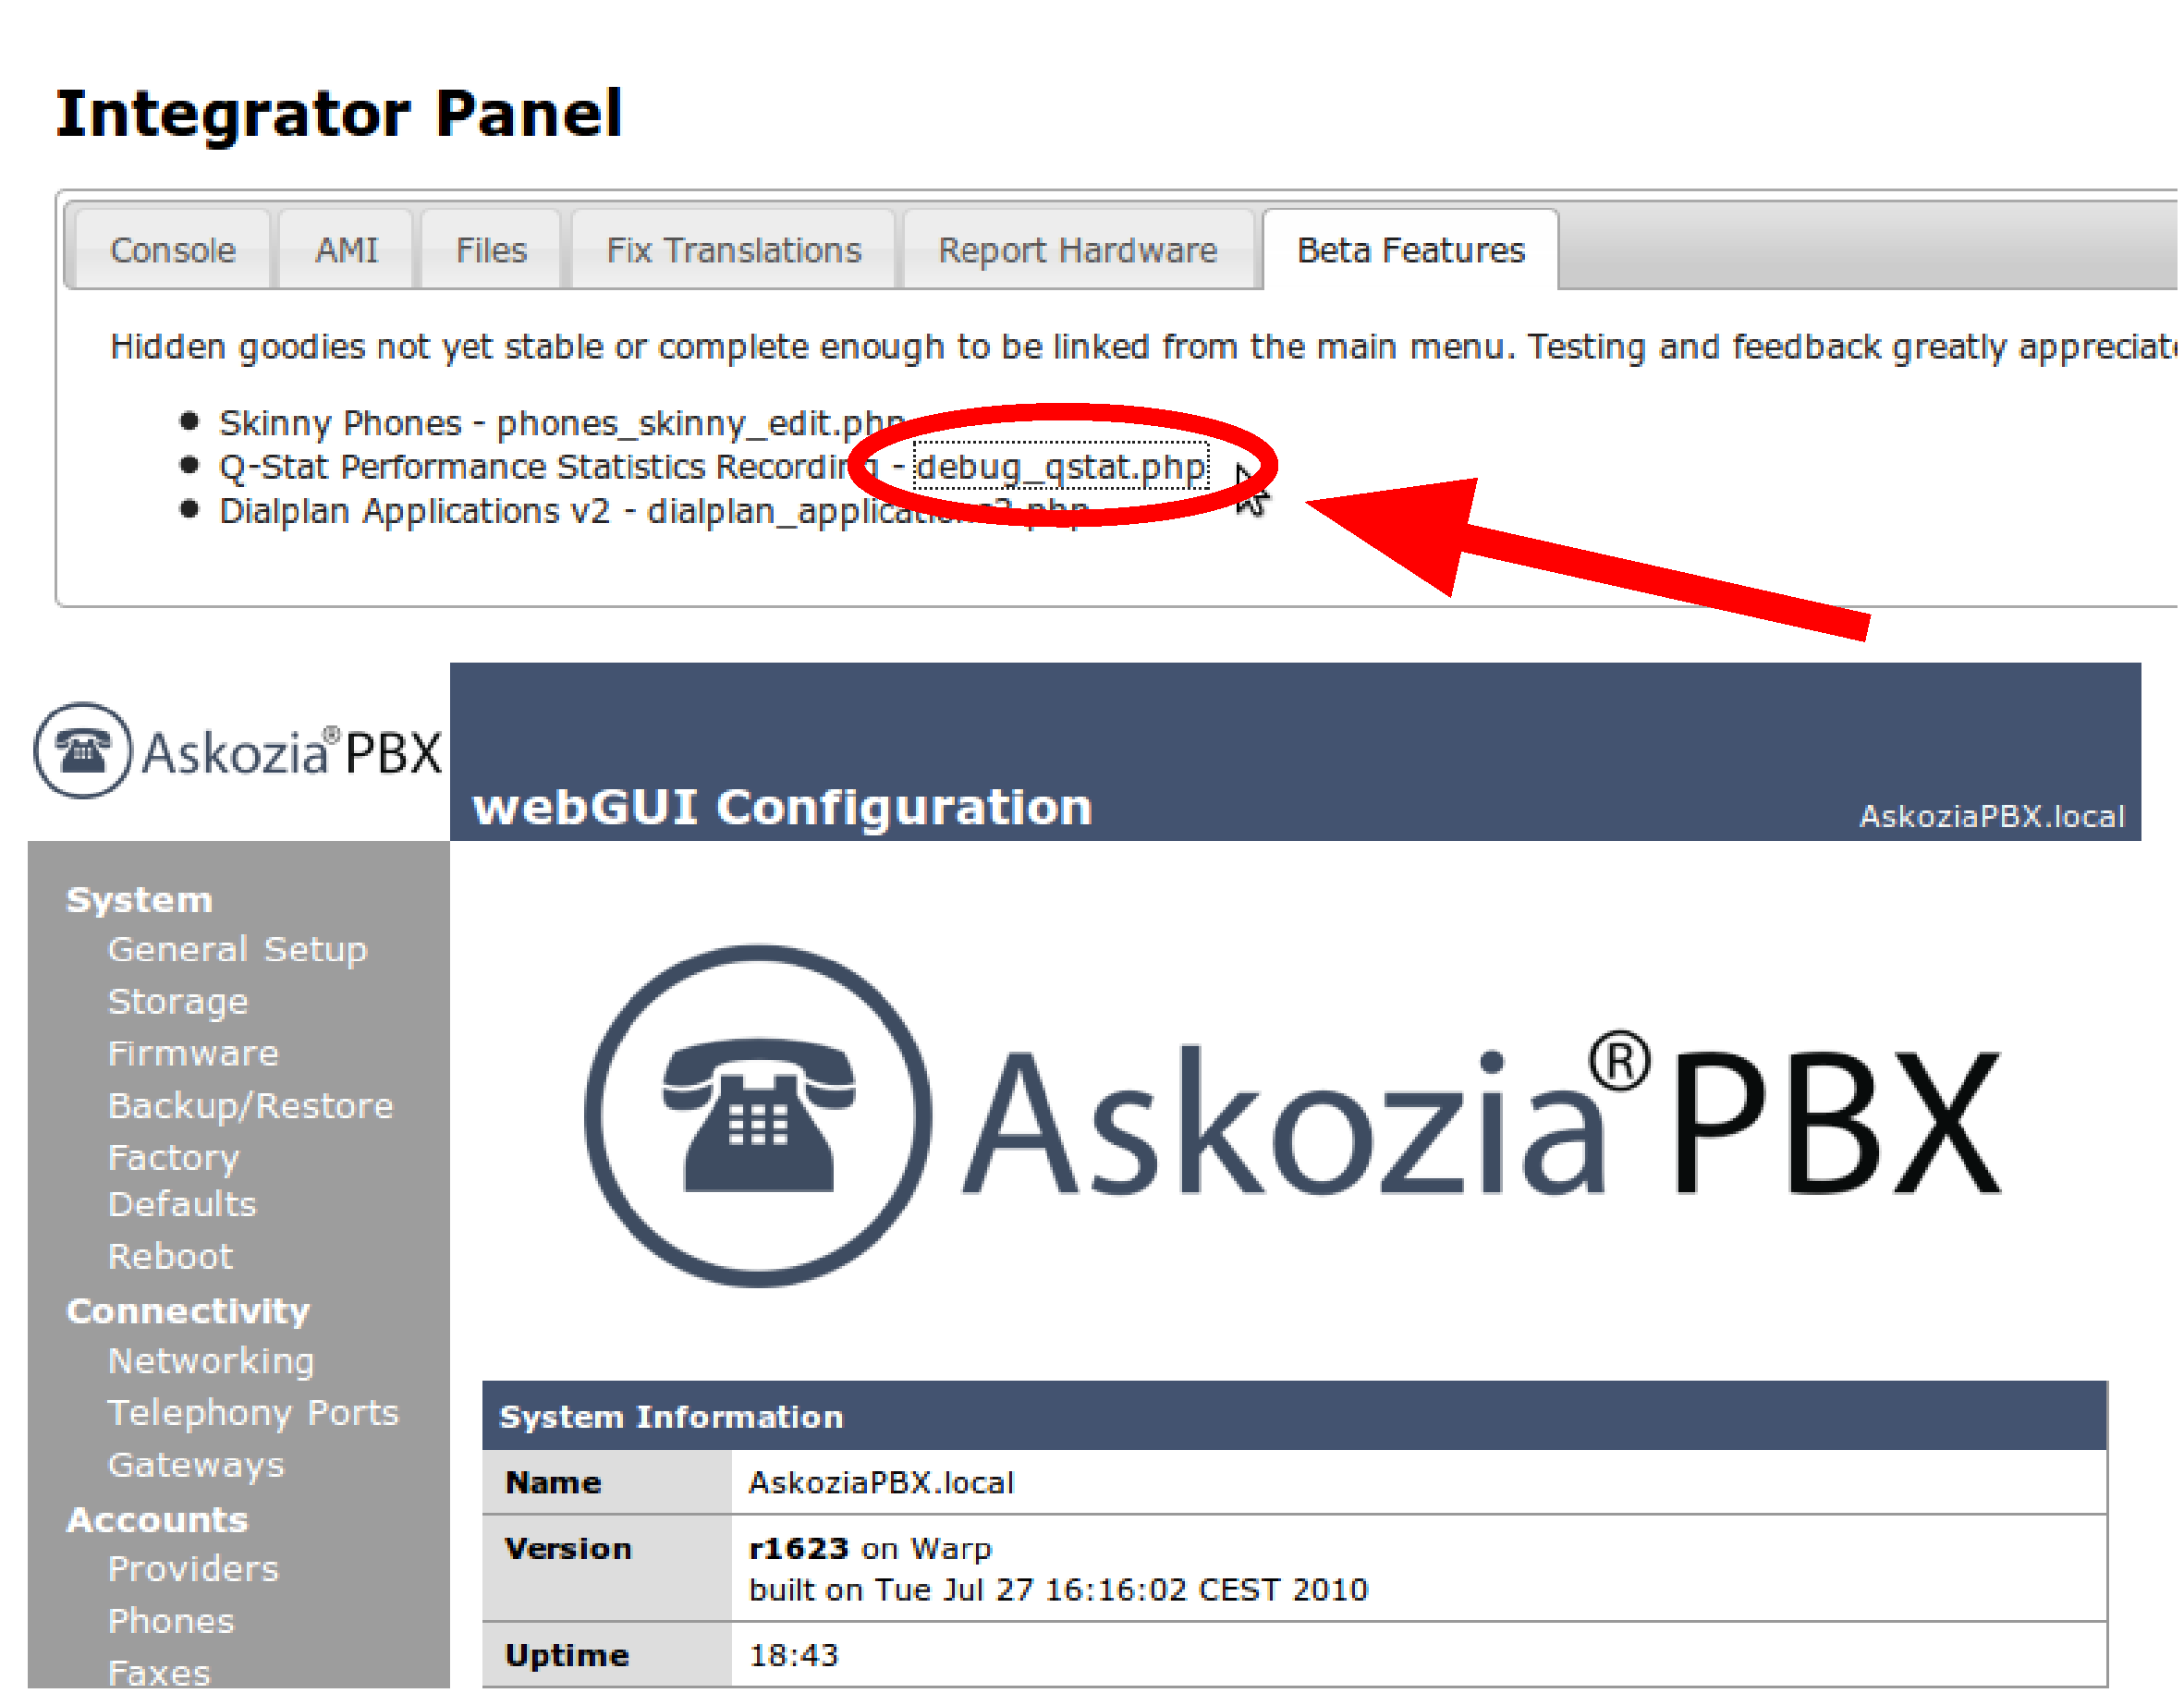
\includegraphics [width=16cm] {qstat-1.pdf}
\caption{Starting qstat manually}
\end{figure}

On the debug qstat page, there is only one button labelled with \texttt{Start}. So, a click on this button starts CPU load
recording by qstat. The button changes top \texttt{Stop} automatically and terminates CPU load recording by clicking on it.
After this, there appears a downloadable file (... .qstat) on the webpage. It contains the recorded qstat data and looks like this:

\begin{figure} [!ht]
\centering
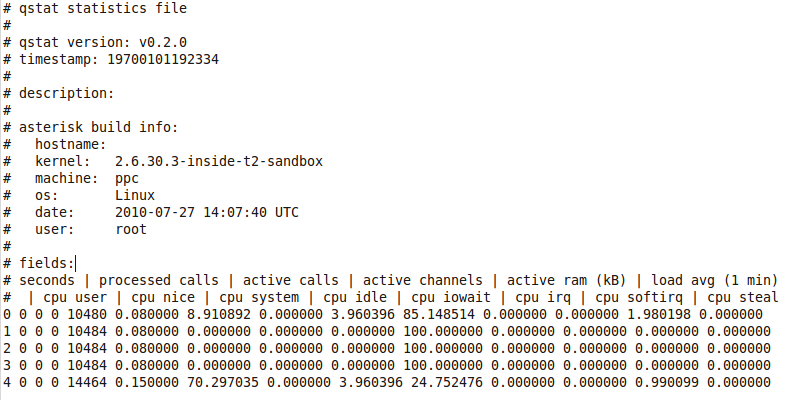
\includegraphics [width=17cm] {qstat-2}
\caption{QStat results}
\end{figure}

The recorded data comprise multiple CPU load values. The script uses the CPU idle time by subtracting it from 100. They were
verified by using \texttt{top} on the AskoziaPBX.

\begin{appendix}
\section{Appendix}
\label{sec:appendix}

%%%%%%%%%%%%%%%%%%%%%%%%%%%%%%%%%%%
\subsection{Developers Parameters}%
%%%%%%%%%%%%%%%%%%%%%%%%%%%%%%%%%%%
\begin {description}

\item {\texttt{-{}-askozia-confpage=<string>}} \newline
Name of the PHP page for downloading/uploading the XML Configuration file
\newline Default: \texttt{system\_backup.php}
\newline Example: \texttt{-{}-askozia-confpage=system\_backup.php}

\item {\texttt{-{}-askozia-realm=<string>}} \newline
Name of the authentication-realm of the AskoziaPBX.
\newline Default: \texttt{Web Server Authentication}
\newline Example: \texttt{-{}-askozia-realm='Web Server Authentication'}

\item {\texttt{-{}-sipp-path=<string>}} \newline
This parameter allows one to override the sipp executable which is used to execute the performance tests.
It is recommended to use the supplied version because it provides a standardized test base.
\newline Default: \texttt{./PERF\_TESTS/sipp} or, if not existing, the result of \texttt{which sipp}
\newline E.g. \texttt{-{}-sipp-path=../sipp} or \texttt{-{}-sipp-path=/tmp/sipp}

\item {\texttt{-{}-two-party-user-file=<string>}} \newline
For executing two-way tests with sipp, there has to be a so-called injection file.
This is a csv file which is used by sipp for generating multiple calls automaticly.
It is created by the script and contains all needed information (and not more)
for sipp. It is possible to change the filepath and -name of this file by specifying
this parameter and may be absolute or relative.
\newline Default: \texttt{./results/<testname>/Users\_two-way.csv}
\newline E.g. \texttt{-{}-users-2way-file=../Users\_two-way.csv}
\newline or \texttt{-{}-users-2way-file=/tmp/Users\_two-way.csv}

\item {\texttt{-{}-participants-user-file=<string>}} \newline
Please have a look at the parameter \texttt{-{}-users-2way-file}.
This parameter is the same only for conference tests with fixed number of rooms.
\newline Default: \texttt{./results/<testname>/Users\_conf\_room.csv}
\newline E.g. \texttt{-{}-users-conf-room-file=../Users\_conf\_room.csv}
\newline or \texttt{-{}-users-conf-room-file=/tmp/Users\_conf\_room.csv}

\item {\texttt{-{}-room-user-file=<string>}} \newline
Please have a look at the parameter \texttt{-{}-users-2way-file}.
This parameter is the same only for conference tests with fixed number of calls.
\newline Default: \texttt{./results/<testname>/Users\_conf\_call.csv}
\newline E.g. \texttt{-{}-users-conf-call-file=../Users\_conf\_call.csv}
\newline or \texttt{-{}-users-conf-call-file=/tmp/Users\_conf\_call.csv}

\item {\texttt{-{}-reg-scen=<string>}} \newline
This parameter specifies the path to the register scenario used by sipp.
The register scenario is needed for two-way tests only.
For more information, please have a look at chapter \ref{sec:two-way}.
\newline Default: \texttt{./PERF\_TEST\_FILES/Register.xml}
\newline E.g. \texttt{-{}-reg-scen=../Register.xml} or \texttt{-{}-reg-scen=/tmp/Register.xml}

\item {\texttt{-{}-dereg-scen=<string>}} \newline
This parameter specifies the path to the deregister scenario used by sipp.
The deregister scenario is needed for two-way tests only.
For more information, please have a look at chapter \ref{sec:two-way}.
\newline Default: \texttt{./PERF\_TEST\_FILES/Deregister.xml}
\newline E.g. \texttt{-{}-dereg-scen=../Deregister.xml} or \texttt{-{}-dereg-scen=/tmp/Deregister.xml}

\item {\texttt{-{}-acc-scen=<string>}} \newline
This parameter specifies the path to the accept scenario used by sipp.
The accept scenario is needed for two-way tests only.
For more information, please have a look at chapter \ref{sec:two-way}.
\newline Default: \texttt{./PERF\_TEST\_FILES/Accept.xml}
\newline E.g. \texttt{-{}-acc-scen=../Accept.xml} or \texttt{-{}-acc-scen=/tmp/Accept.xml}

\item {\texttt{-{}-inv-scen=<string>}} \newline
This parameter specifies the path to the invite scneario used by sipp.
The invite scenario is needed for every test type.
For more information, please have a look at the description of the
different testtypes (chapters \ref{sec:two-way}, \ref{sec:conf-call} and \ref{sec:conf-room}).
\newline Default: \texttt{./PERF\_TEST\_Files/Invite.xml}
\newline E.g. \texttt{-{}-inv-scen=../Invite.xml} or \texttt{-{}-inv-scen=/tmp/Invite.xml}

\item {\texttt{-{}-sip-src-port=<number>}} \newline
Port of the local computer (testcomputer) to communicate with Askozia.
It is used for User A in two-way tests and for all users in conference tests.
During the tests, there was a softphone running in background for communication
in the office. Because of this, sipp was not able to reserve the usual sip port 5060.
\newline Default: \texttt{5061}
\newline E.g. \texttt{-{}-sip-src-port=5061}

\item {\texttt{-{}-sip-dst-port=<number>}} \newline
Port of the local computer (testcomputer) to communicate with Askozia,
but this time only for User B in two-way tests. The first sipp process
(User A) blocks one port for communication with AskoziaPBX,
so the second sipp process (User B) needs another one to talk to Askozia.
This is necessary for two-way tests only.
\newline Default: \texttt{5062}
\newline E.g. \texttt{-{}-sip-dst-port=5062}

\item {\texttt{-{}-rtp-src-port=<number>}} \newline
Port of the local computer for establishing RTP streams between the local testcomputer
and AskoziaPBX. This one is used by User A of two-way tests and by all users of
conference tests. Sipp was not able to use the standard port because of a
softphone running on the testcomputer in background.
\newline Default: \texttt{6020}
\newline E.g. \texttt{-{}-rtp-src-port=6020}

\item {\texttt{-{}-rtp-dst-port=<number>}} \newline
Port of the local computer for establishing RTP streams between the local testcomputer
and AskoziaPBX. This one is used by User B of two-way tests only, so it not needed
for conference testing.
\newline Default: \texttt{6030}
\newline E.g. \texttt{-{}-rtp-dst-port=6030}

\item {\texttt{-{}-restore=<string>}} \newline
After the test, the AskoziaPBX is strongly reconfigured. There are possibly hundreds
of testusers and some new conference rooms. To avoid cleaning up by hand, this parameter
helps to reconfigure the box after the test. There are three possible values:
\begin{description}
	\item [none] The AskoziaPBX is not reconfigured.
	\item [old-config] The AskoziaPBX is restored with the config existing before the test.
	\item [factory-defaults] The AskoziaPBX is set to factory-defaults.
\end{description}
Default: \texttt{old-config}
\newline E.g. \texttt{-{}-restore=none} or \texttt{-{}-restore=factory-defaults}

\item {\texttt{-{}-gnuplot-exe=<string>}} \newline
The path to the gnuplot executable for drawing graphs of the results at the end of the test.
Has to be installed (\texttt{which gnuplot} determines path) or specified if the graphs
should be drawed. If not installed and specified (undefined), there is no possibility to
draw the graphs. The test can nevertheless be executed.
\newline Default: result of \texttt{which gnuplot} or, if not existing, undefined
\newline E.g. \texttt{-{}-gnuplot-exe=../gnuplot} or \texttt{-{}-gnuplot-exe=/tmp/gnuplot}

\item {\texttt{-{}-two-party-user-file=<string>}} \newline
For executing two-way tests with sipp, there has to be a so-called injection file.
This is a csv file which is used by sipp for generating multiple calls automaticly.
It is created by the script and contains all needed information (and not more)
for sipp. It is possible to change the filepath and -name of this file by specifying
this parameter and may be absolute or relative.
\newline Default: \texttt{./results/<testname>/Users\_two-way.csv}
\newline E.g. \texttt{-{}-users-2way-file=../Users\_two-way.csv}
\newline or \texttt{-{}-users-2way-file=/tmp/Users\_two-way.csv}

\item {\texttt{-{}-participants-user-file=<string>}} \newline
Please have a look at the parameter \texttt{-{}-users-2way-file}.
This parameter is the same only for conference tests with fixed number of rooms.
\newline Default: \texttt{./results/<testname>/Users\_conf\_room.csv}
\newline E.g. \texttt{-{}-users-conf-room-file=../Users\_conf\_room.csv}
\newline or \texttt{-{}-users-conf-room-file=/tmp/Users\_conf\_room.csv}

\item {\texttt{-{}-room-user-file=<string>}} \newline
Please have a look at the parameter \texttt{-{}-users-2way-file}.
This parameter is the same only for conference tests with fixed number of calls.
\newline Default: \texttt{./results/<testname>/Users\_conf\_call.csv}
\newline E.g. \texttt{-{}-users-conf-call-file=../Users\_conf\_call.csv}
\newline or \texttt{-{}-users-conf-call-file=/tmp/Users\_conf\_call.csv}

\item {\texttt{-{}-reg-scen=<string>}} \newline
This parameter specifies the path to the register scenario used by sipp.
The register scenario is needed for two-way tests only.
For more information, please have a look at chapter \ref{sec:two-way}.
\newline Default: \texttt{./PERF\_TEST\_FILES/Register.xml}
\newline E.g. \texttt{-{}-reg-scen=../Register.xml} or \texttt{-{}-reg-scen=/tmp/Register.xml}

\item {\texttt{-{}-dereg-scen=<string>}} \newline
This parameter specifies the path to the deregister scenario used by sipp.
The deregister scenario is needed for two-way tests only.
For more information, please have a look at chapter \ref{sec:two-way}.
\newline Default: \texttt{./PERF\_TEST\_FILES/Deregister.xml}
\newline E.g. \texttt{-{}-dereg-scen=../Deregister.xml} or \texttt{-{}-dereg-scen=/tmp/Deregister.xml}

\item {\texttt{-{}-acc-scen=<string>}} \newline
This parameter specifies the path to the accept scenario used by sipp.
The accept scenario is needed for two-way tests only.
For more information, please have a look at chapter \ref{sec:two-way}.
\newline Default: \texttt{./PERF\_TEST\_FILES/Accept.xml}
\newline E.g. \texttt{-{}-acc-scen=../Accept.xml} or \texttt{-{}-acc-scen=/tmp/Accept.xml}

\item {\texttt{-{}-inv-scen=<string>}} \newline
This parameter specifies the path to the invite scneario used by sipp.
The invite scenario is needed for every test type.
For more information, please have a look at the description of the
different testtypes (chapters \ref{sec:two-way}, \ref{sec:conf-call} and \ref{sec:conf-room}).
\newline Default: \texttt{./PERF\_TEST\_Files/Invite.xml}
\newline E.g. \texttt{-{}-inv-scen=../Invite.xml} or \texttt{-{}-inv-scen=/tmp/Invite.xml}

\item {\texttt{-{}-sip-src-port=<number>}} \newline
Port of the local computer (testcomputer) to communicate with Askozia.
It is used for User A in two-way tests and for all users in conference tests.
During the tests, there was a softphone running in background for communication
in the office. Because of this, sipp was not able to reserve the usual sip port 5060.
\newline Default: \texttt{5061}
\newline E.g. \texttt{-{}-sip-src-port=5061}

\item {\texttt{-{}-sip-dst-port=<number>}} \newline
Port of the local computer (testcomputer) to communicate with Askozia,
but this time only for User B in two-way tests. The first sipp process
(User A) blocks one port for communication with AskoziaPBX,
so the second sipp process (User B) needs another one to talk to Askozia.
This is necessary for two-way tests only.
\newline Default: \texttt{5062}
\newline E.g. \texttt{-{}-sip-dst-port=5062}

\item {\texttt{-{}-rtp-src-port=<number>}} \newline
Port of the local computer for establishing RTP streams between the local testcomputer
and AskoziaPBX. This one is used by User A of two-way tests and by all users of
conference tests. Sipp was not able to use the standard port because of a
softphone running on the testcomputer in background.
\newline Default: \texttt{6020}
\newline E.g. \texttt{-{}-rtp-src-port=6020}

\item {\texttt{-{}-rtp-dst-port=<number>}} \newline
Port of the local computer for establishing RTP streams between the local testcomputer
and AskoziaPBX. This one is used by User B of two-way tests only, so it not needed
for conference testing.
\newline Default: \texttt{6030}
\newline E.g. \texttt{-{}-rtp-dst-port=6030}

\item {\texttt{-{}-restore=<string>}} \newline
After the test, the AskoziaPBX is strongly reconfigured. There are possibly hundreds
of testusers and some new conference rooms. To avoid cleaning up by hand, this parameter
helps to reconfigure the box after the test. There are three possible values:
	\begin{description}
	\item [none] The AskoziaPBX is not reconfigured.
	\item [old-config] The AskoziaPBX is restored with the config existing before the test.
	\item [factory-defaults] The AskoziaPBX is set to factory-defaults.
	\end{description}
Default: \texttt{old-config}
\newline E.g. \texttt{-{}-restore=none} or \texttt{-{}-restore=factory-defaults}
\end{description}

\subsection{XML Scenarios}
\subsubsection{REGISTER Scenario}
\subsubsection{De-REGISTER Scenario}
\subsubsection{INVITE Scenario}
\subsubsection{ACCEPT Scenario}

\subsection{Example Configuration File}

\subsection{SIPP Manpage}


\end{appendix}
\bibliographystyle {natdin}
\bibliography{/Users/t001/Documents/praxissemester/uboot-doku/referenz.bib}
%\printbibliography[heading=printed,type=book]
%\printbibliography[heading=standards,type=misc]
%\printbibliography[heading=url,type=online] 
\nocite{*}
\end {document}

